\documentclass[a4paper, 12pt]{article}

\usepackage{babel}
\usepackage{enumitem}
\usepackage{times}
\usepackage{graphicx}
\usepackage{geometry}
	\geometry{left = 4cm, top = 4cm, right = 3cm, bottom = 3cm}
\usepackage{float}
\usepackage{setspace}
	\setstretch{1.5}
\usepackage{listings}


\begin{document}
\title{\huge\textbf{Tugas Besar Database II \\
Pembuatan Aplikasi catering}}
\date{}

\maketitle


\begin{figure}[!ht]
\begin{center}

\includegraphics[width = 6cm, height = 6cm]{poltekpos.JPG}
\end{center}
\end{figure}

\begin{center}
\vspace{1cm}
Disusun oleh :\\
Putri Nella\\
D4 TI 2C\\
1.18.4.017\\
\vspace{1cm}
\textbf{PROGRAM DIPLOMA IV POLITEKNIK POS INDONESIA} \linebreak
\textbf{POLITEKNIK POS INDONESIA} \linebreak
\textbf{BANDUNG}\linebreak
\textbf{2019}

\end{center}


\thispagestyle{empty}

\chapter{PENYUSUNAN LAPORAN}
\section{Tujuan}
Untuk	 melaporkan	 jalannya	 pekerjan	 Proyek	 serta	 hasil	 yang	 diperoleh,	 mahasiswa	diwajibkan	menyusun	laporan	pekerjaan	Proyek.

\section{Ketentuan Penyusunan Laporan}
\subsection{Format Laporan}
Laporan	Proyek	hendaknya	berisi	:

\begin{enumerate}
\item \textbf{ Bagian Awal}
	\begin{itemize}
		\item Lembar	Muka	
		\item Lembar Pengesahan
		\item Surat	Pernyataan	Tidak	Melakukan	Plagiarisme
	 \item Abstrak	(dalam	Bahasa	Indonesia)
	 \item Abstract(dalam	Bahasa	Inggris)
	 \item Kata	Pengantar
	 \item Daftar	Isi	termasuk	:
 \begin{enumerate}[label=(\alph*)]
 
	\item Daftar	Gambar
	\item Daftar	Tabel
	\item Daftar	Simbol
	\item Daftar	Singkatan	
	\item Daftar	Lampiran
 \end{enumerate}
 \end{itemize}
 
\item \textbf{Bagian Isi}
 	\par \textbf{BAB	I PENDAHULUAN}
 	
 	\begin{enumerate} [label=1.\arabic*]
 	\item \textbf{ Latar	Belakang} \par 
Berisi	ulasan	ringkas	mengenai	keadaan/kondisi	yang	ada	dan	
kekurangan	 dari	 sistem	 yang	 diamati	 sehingga	 muncul	 topik	
yang	diambil.

\item \textbf{ Identifikasi	Masalah} \par 
Berisi	 berbagai	 masalah	 yang	 sudah	 dikenali	 dan	 	 akan diberikan	 solusinya	 melalui	 fungsi	 dari	 sistem/aplikasi/alat	yang	akan	dibuat.

\item \textbf{Tujuan} \par
Berisi	tujuan	untuk	apa	sistem/aplikasi/alat	itu	dibuat.

\item \textbf{ Ruang	Lingkup	} \par
Berisi	batasan-batasan	proyek	atau	cakupan	aplikasi	yang	akan	
dibangun.

\item \textbf{ Sistematika	Penulisan} \par
Menjelaskan	isi	yang	ada	di	laporan	proyek.\\
 
 	\end{enumerate}
 	
 \par \textbf{BAB II LANDASAN TEORI} \par 
 
 	Uraian	 \textbf{tentang	 teori yang	 mendukung} Objek	 PROYEK 2.	 \textbf{Harus	jelas	 sumber	 rujukannya	 dari	 mana}. Sumber	 yang	 baik	 adalah	jurnal	 ilmiah,	 artikel	 ilmiah,	 buku,	 dll.	 \textit{\textbf{Disarankan	 untuk	 tidak	mengambil	sumber	seperti	WebBlog,	Wikipedia,	dll.}} \\
 	
 	\par \textbf{BAB III ANALISIS DAN PERANCANGAN} \par 
 	\textit{\textbf{Analisis}} : \par 
 	Proses	 untuk	 menentukan	 bentuk	 dari	 kebutuhan	
sistem/aplikasi/alat	 baik	 berupa	 kebutuhan	 pada	 saat	membangun	
maupun	pada	saat	Implementasi.

	\textit{\textbf{Perancangan}}: \par 
	Penjelasan	 perancangan	 	 sistem/aplikasi/alat	 	 yang	 akan	 dibuat	terdiri	dari	perancangan	alir	program \textit{\textbf{(Flow	Chart)}}	, algoritma,	data,	maupun	perancangan	input/output	sistem/aplikasi/alat.		
 	
	
	\begin{enumerate} [label=3.\arabic*]
		\item Analisis
			\begin{enumerate} [label=3.1.\arabic*]
				\item Analisis	Sistem	yang	Sedang	Berjalan
					\begin{enumerate} [label=3.1.1.\arabic*]
						\item Analisis	Prosedur/ \textit{Flow	Map} yang								  berjalan
						\item Analisis	Dokumen	yang digunakan
					\end{enumerate}
				\item Analisis	Sistem	yang	akan	Dibangun
					\begin{enumerate} [label=3.1.2.\arabic*]
						\item Analisis	Kebutuhan	Aplikasi
						\item Analisis	Kebutuhan	Perangkat	lunak									  dan	Perangkat Keras
					\end{enumerate}
			\end{enumerate}
			
			
		\item Perancangan \textit{\textbf{(Jika	menggunakan	procedural 					  atau DFD)}}
			\begin{enumerate} [label=3.2.\arabic*]
				\item \textit{Context	Diagram}
				\item \textit {Data	Flow	Diagram} (disertai	tabel									  spesifikasi	Proses)
				\item Kamus	Alir	Data \textit{(Data Dictionary)}
				\item 	Perancangan	 \textit{Database (Sesuaikan	Format							Penulisannya)}
					\begin{enumerate} [label=3.2.4.\arabic*]
						\item \textit{Conceptual	Data	Model}
						\item \textit{Physical	Data	Model}
						\item \textit{Kamus	Data	Tabel (Database)}	
					\end{enumerate}
				\item Struktur Menu
				\item Perancangan Antarmuka
			\end{enumerate}
			
	\end{enumerate}
			
			\begin{enumerate} [label=3.2]
				\item Perancangan \textit{\textbf{(Jika	menggunakan 							  	Object	Oriented UML)}}
			\end{enumerate}
				\begin{enumerate} [label=3.2.\arabic*]
				\item \textit{Use	Case	Diagram}
				\item \textit{Class	Diagram}
				\item \textit{Interaction	Diagram}
				\item \textit{Sequence	Diagram}
				\item \textit{Collaboration	Diagram}
				\item \textit{Activity	Diagram}
				\item \textit{Statechart	Diagram}
				\item \textit{Componen	Diagram}
				\item \textit{Deployment	Diagram}
				\item \textit{Objek	Diagram}
				\item Perancangan \textit{Database (Sesuaikan	Format							  Penulisannya)}
						\begin{enumerate}[label=(\alph*)]
							\item \textit{Conceptual Data Model	(CDM)}
							\item \textit{Physical	Data Model (PDM)}
						\end{enumerate}
				\item Struktur	Menu
				\item Perancangan	Antarmuka
				\end{enumerate} 
				
	\par \textbf{BAB IV IMPLEMENTASI DAN PENGUJIAN} \par 
	\textbf{Implementasi} : \par 
	adalah	sistem/aplikasi/alat	yang	dibuat	dengan	merinci	komponenkomponen	 pendukung	 berupa	 program,	 Lingkungan	 Implementasi, Tampilan	Antarmuka,	Petunjuk	Pemakaian,	Petunjuk	Instalasi.
	
	\textbf{Pengujian} : \par 
	Adalah	 Cara	 untuk	 mengetahui	 apakah	 sistem/aplikasi/alat	 yang dibuat	sesuai	dengan	rancangan	dan	menuliskan	hasil	ujinya.
\textit{Jika	 anda	 membuat	 analisis	 sistem/aplikasi,	 maka	 harus	 seperti berikut:}
	
	\begin{enumerate} [label=4.\arabic*]
		\item Lingkungan	Implementasi \par 	
		Berisi	 perangkat	 lunak	 dan	 perangkat	 keras	 apa	 saja yang	digunakan	 sewaktu	 perancangan	 aplikasi	 berupa	 sistem	operasi,	database,	prosesor,	memory,	space	harddisk	dan	lain-lain	sesuai	dengan	kebutuhan serta	perangkat	pendukungnya.
		
		\item Pembahasan	Hasil	Implementasi \par 
		Berisi	 uraian	 hasil	 implementasi	 sistem	 yang	 disesuaikan	dengan	 tujuan	 pembuatan	 sistem.	 Jelaskan bahwa	 masalah	 yang	teridentifikasi	 pada	 identifikasi	 masalah yang berada	 di	 bab	 1	 telah	terseleseaikan, dan	 tujuan	 dari	 pelaksanaan	 proyek	telah tercapai. Penjelasan	dibantu	dengan	Tampilan	Antarmuka	aplikasi.
		
		\item Pengujian	dan	hasil	Pengujian \par 
		Berisi	identifikasi	 pengujian,	 rencana	 pengujian,	 deskripsi dan hasil	uji.	Metoda	yang	digunakan	misalnya \textit{white	box testing} dan \textit{	black	box	testing}
		
	\end{enumerate}	 
	
	
	
	\par \textbf{BAB V KESIMPULAN	DAN	SARAN} \par 
	
	\begin{enumerate} [label=5.\arabic*]
		\item \textbf{Kesimpulan} : \par 
				berisi	pencapaian	tujuan	dari	sistem/aplikasi/alat	                yang	dibuat.
		\item \textbf{Saran} : \par 
				berisi	hal-hal	atau	tujuan	dari	pembuatan	sistem/aplikasi/alat	yang dirasa	belum	sempurna	atau	 tidak	 tercapai.	Saran	juga	bisa	berupa	kondisi	 implementasi	 yang	 optimal	 bagi	 sistem/aplikasi/alat	 yang dibuat.
	\end{enumerate}
			
			
\item Bagian Akhir
 \begin{itemize}
 	\item Daftar	Pustaka		(Lampiran	8)
 	\item Lampiran
 	\item Tabel-tabel
 \end{itemize} 
 		 	
\end{enumerate}

\section{Ukuran	Kertas	dan	Ukuran	Huruf}

\begin{itemize}
	\item Penulisan	 dan	 ejaan	 menggunakan	 ketentuan	 bahasa	 Indonesia	 yang	 baik	 dan	
benar;
	\item Penulisan	diketik	dengan	komputer,	dengan	ketentuan	:
		\begin{enumerate}
			\item Jarak	1,5 spasi ;
			\item Lebar	sembir	kiri	4	cm ;
			\item Lebar	sembir	kanan	2,5	cm ;
			\item Lebar	sembir	atas	3	cm ;
			\item Lebar	sembir	bawah	3	cm ;
			\item Ukuran	Font	adalah	\textit{Times	New	Roman} 12	Kecuali	untuk	judul	bab	menggunakan	\textit{Times New Roman} dengan	ukuran	14.
		\end{enumerate}
		
	\item Ukuran	buku	adalah	A4	(21	x	29,7	Cm),	dengan	berat	kertas	80	gram;
	
	\item Sampul	depan	adalah	mika/softcover mika,	dengan	ketentuan	seperti	ini	:
		\begin{enumerate}
			\item Proposal	Proyek   \qquad \qquad \enspace : Mika Transparan .
			\item Buku Laporan Proyek \qquad : \textit{Softcover} Merah Omega 17.
		\end{enumerate}
		
		
\section{Ketentuan	Khusus}
	\begin{enumerate}
		\item \textbf{Abstrak} : Jarak	 1	 spasi,	 maksimal	 1	 halaman,	 font	 12,	 italic,	 maksimum	 200	 kata.
Hanya	1	paragraf. Kata	kunci	minimal	5.

		\item Penomoran	 tabel	 dilakukan	 dengan	 menyebutkan	 nomor	 bab,	 diikuti	 nomor	 urut	tabelnya	pada	bab	tersebut,	misalnya	Tabel	3.7,	artinya	tabel	nomor 7	di	bab	3.	Judul	
tabel	 diletakkan	 di	 atas	 tabel,	 penulisannya	 dengan	 huruf	 kapital	 di	 awal	 kata.	 Bila	tabel	 lebih	 panjang	 dari	 halaman,	 maka	 sambungan	 tabel	 pada	 halaman	 berikutnya	
diberi	judul	dengan	tulisan	: \textbf{(Lanjutan)}
		\item Tulisan	di	dalam	tabel	Jarak	1 spasi,	ukuran	huruf kurang	atau	sama	dengan \textit{font} 10 ( $\leq \textit{font}  10$). 	Judul	tabel	disimpan diatas	table	tanpa	jarak	spasi.
		
		\item Penomoran	 gambar	 dilakukan	 dengan	menyebutkan	 nomor	 bab,	 diikuti	 nomor	 urut	gambarnya	pada	bab	tersebut,	misalnya		Gambar	2.5,	artinya	gambar	nomor	5	di	bab	
2.			 Judul	gambar	diletakkan	di	bawah	gambar,	penulisannya	dengan	huruf	kapital	di	awal	kata.

		\item Penomoran	 halaman	 dimulai	 dari	 nomor	 1	 untuk	 tiap	 bab	 atau	 lampiran,	 dengan	
ketentuan	sebagai	berikut:	\\
			Penomoran	 dari	 bab	 1	 sampai	 bab	 5	 dimulai	 dari	 halaman	 1	 sampai	 selanjutnya	sekuensial	tanpa	menggunakan	bab	contoh	;	pada	awal	bab	2,	jika	bab	1	sebanyak	10	halaman,	maka	bab	2	dimulai	dengan	halaman	11	dst. .
			
		\item Penomoran	 halaman	 judul,	 buku	 laporan,	 halaman	 	 persetujuan,	 Daftar	 Isi,	 Daftar	Tabel,	dan	Daftar		Gambar	menggunakan	i,		ii,		iii,	…..	(angka	romawi	kecil).
		
		\item Setelah	Buku	laporan	 ditandatangani	 oleh	 pembimbing	 dan	 penguji	 seminar/sidang,	
maka	harus	di	buatkan	Jurnal	dengan	jumlah	halaman	maksimum	6	halaman.

		\item \textit{Softcopy} dari	jurnal, \textit{software} dan	laporan	disimpan	dalam	sebuah	CD	dan	disertakan	
ke	dalam	laporan di	beri	judul	serta	penulis	di	label	CD	nya.

	\end{enumerate}
\end{itemize}

\section{Status	Buku}
\begin{enumerate}
	\item Status Buku \par 
		Buku	 yang	 memenuhi	 persyaratan	 untuk	 sidang Proyek	 adalah	 buku	 yang	 telah	
selesai	 100 \%.	 Penjilidan	 buku	 sebelum	 sidang menggunakan	 penjepit	 dan	 sampul	plastik	mika	warna	Transparan;

	\item Setelah	Sidang \par 
		Buku	 yang	 memenuhi	 persyaratan	 untuk	 keluarnya	 nilai	 adalah	 buku	 yang	 telah	selesai	 100 \%	 (telah	 diperbaiki,	 jika	 ada	 tugas	 perbaikan).Penjilidan	 	 buku	 setelah	sidang dan	 setelah	 melalui	 perbaikan	 adalah	 jilid	 punggung	 disertai	 halaman	pembatas	bab	warna	merah	seperti	pita	pembatas	warna	merah.	
		
\end{enumerate}

\section{Distribusi	Buku}
Jumlah	 salinan	 laporan	 Proyek	 untuk	 keperluan	 sidang Proyek	 adalah	 3	 \textit{copy},	 dengan	distribusi	sebagai	berikut	:

\begin{enumerate}
	\item Pembimbing/Ketua	Penguji \quad (1 copy)
	\item Anggota	Penguji \qquad \qquad \qquad(1 copy)
	\item Mahasiswa \qquad \qquad \qquad \enspace \quad \quad(1 copy)
\end{enumerate}

Jumlah	salinan	buku	laporan	Proyek		adalah	4	 (empat) \textit{	 copy},	dengan	distribusi	sebagai	berikut	:

\begin{table}[H]
\label{tab:my-table}
\begin{tabular}{lll}
1 & Pembimbing & (1 CD) \\ \\
2 & Perpustakaan	Politeknik	Pos	Indonesia & (1 Buku dan CD ) \\ \\
3 & Mahasiswa & (1 Buku) \\ \\
4 & \multicolumn{2}{l}{\begin{tabular}[c]{@{}l@{}}Prodi	(1	 CD yang	 berisi	 jurnal,	 aplikasi	 dan	 laporan) dan	 hardcopy	 jurnal	 1	 buah	\\ tanpa	di	jilid.\end{tabular}}
\end{tabular}
\end{table}

\section{Proses Pembuatan Table}
\begin{center}
    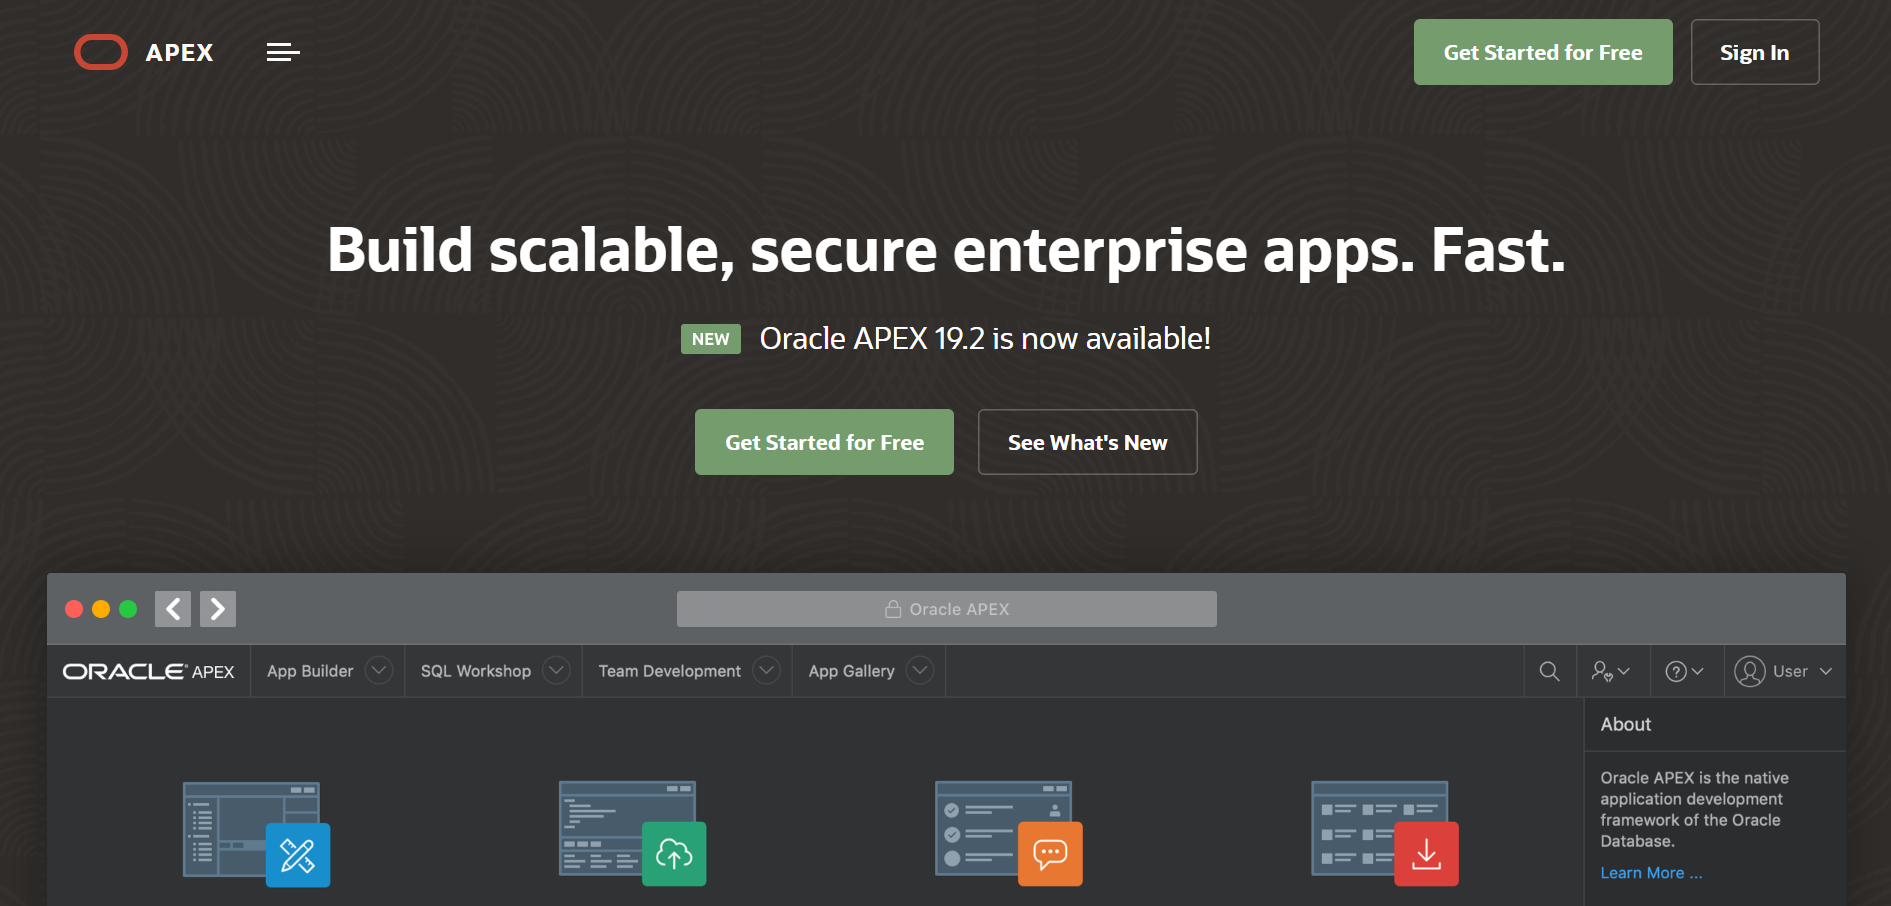
\includegraphics[width=.8\textwidth]{figure/awalan.PNG}
\end{center}
\begin{enumerate}
\item Sebelum membuat table yang berisi data-data,pertama-tama kita masuk ke workspace apex kita dulu.
\begin{center}
    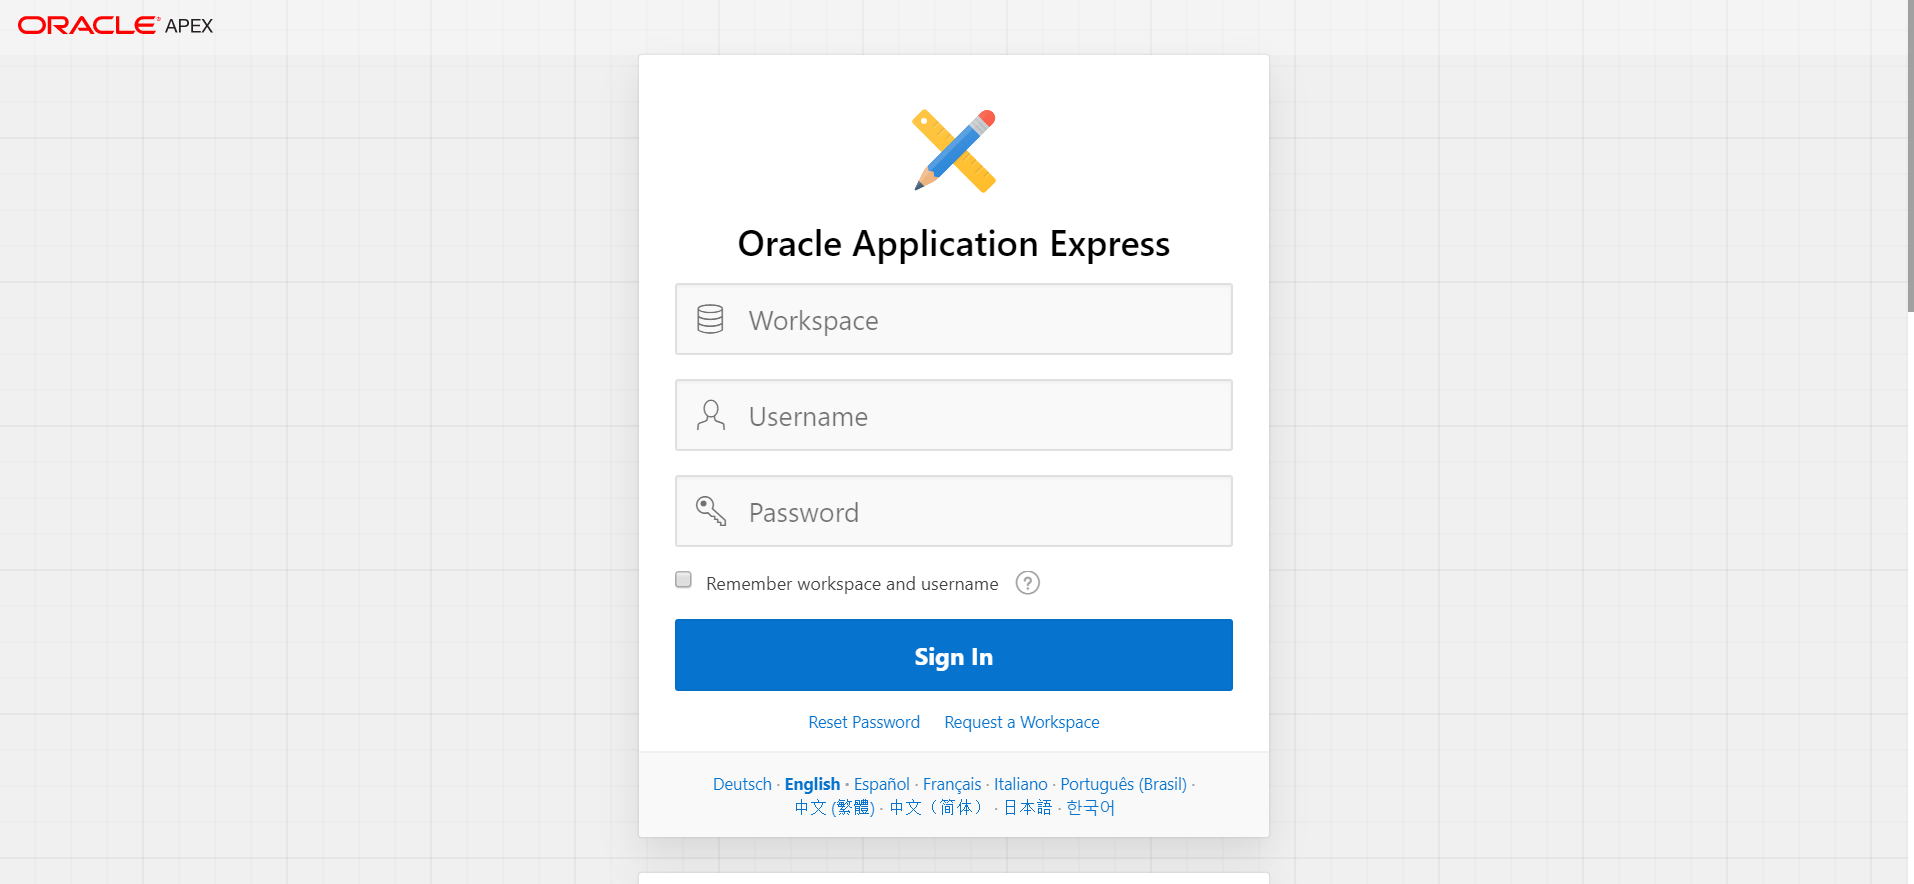
\includegraphics[width=.8\textwidth]{figure/Login.PNG}
\end{center}
\item setelah klik sign in terdapat form login.masukkan nama workspace,username,dan password kita masing masing.
\begin{center}
    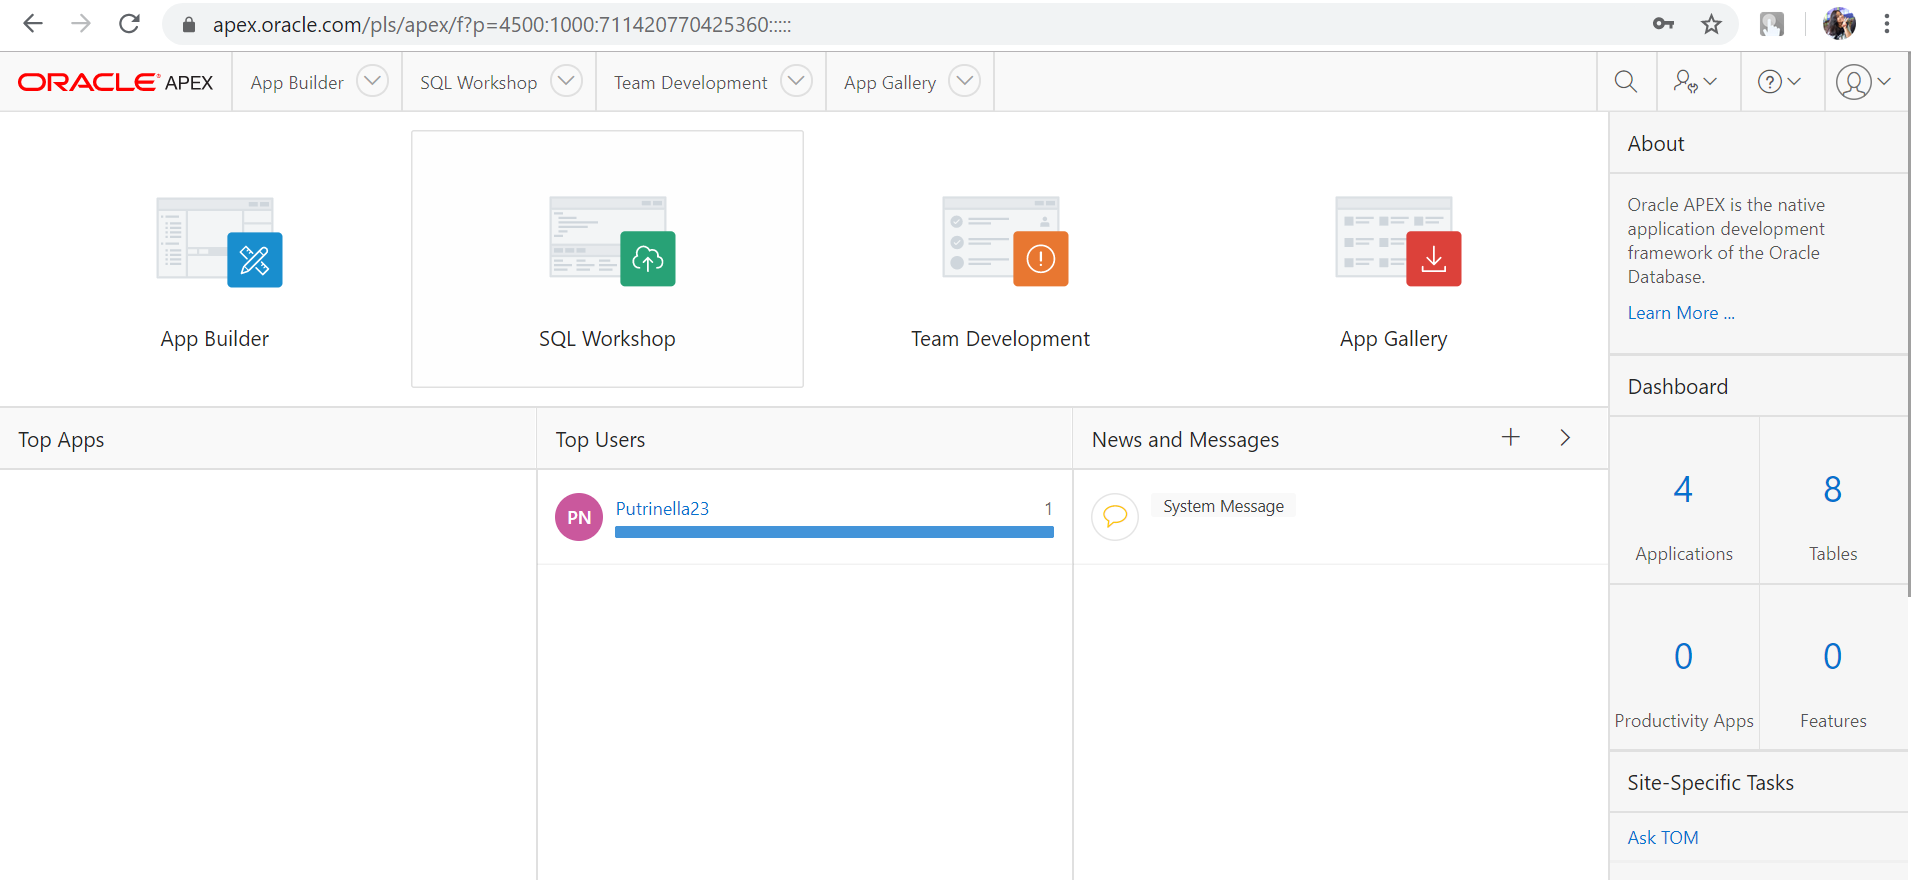
\includegraphics[width=.8\textwidth]{figure/home.PNG}
\end{center}
\item pertama kita buka sql comman pada sql workshop untuk membuat table.
\begin{center}
    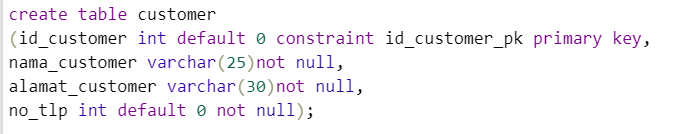
\includegraphics[width=.8\textwidth]{figure/20.PNG}
\end{center}
\item setelah membuka sql command,selanjutanya kita akan mengcreate table costumer sesuai dengan dengan atribut ada id custumer(int),nama custumer(varchar),alamat customer(varchar),no tlp(int) yang akan dibuat dengan fungsi create.
\begin{center}
    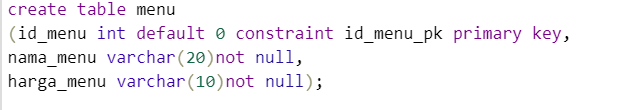
\includegraphics[width=.8\textwidth]{figure/21.PNG}
\end{center}
\item setelah table customer terbentuk,selanjutnya adalah membuat table menu,dengan menggunakan fungsi create.Pada tabel menu terdapat atribut id menu,nama menu,harga menu.
\begin{center}
    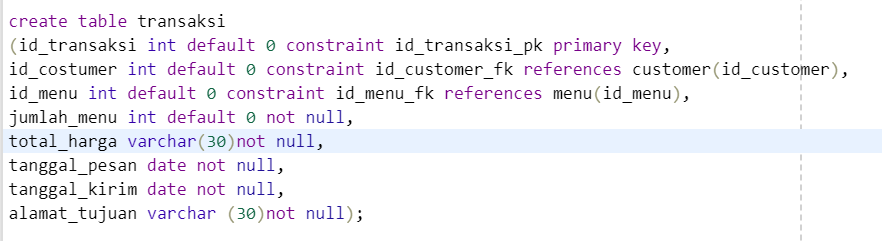
\includegraphics[width=.8\textwidth]{figure/23.PNG}
\end{center}
\item table terakhir yang akan dibuat yaitu tabel transaksi dengan atribut id transaksi sebagai primary key.sedangkan id menu dan id customer sebagai foreign key.pada tabel transaksi terdapat atribut jumlah menu,total harga,tanggal harga,tanggal pesan,tanggal kirim,alamat tujuan.
\begin{center}
    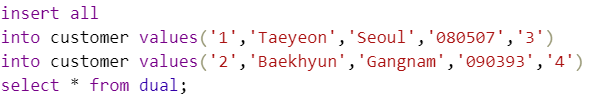
\includegraphics[width=.8\textwidth]{figure/24.PNG}
\end{center}
\item setelah table customer telah terbentuk langkah selanjutnya yaitu memasukkan data menggunakan fungsi insert ke tabel customer.
\begin{center}
    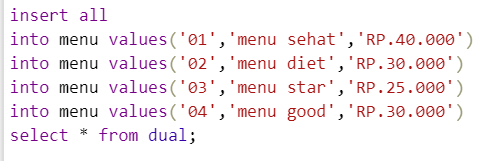
\includegraphics[width=.8\textwidth]{figure/25.PNG}
\end{center}
\item sselanjutnya adalah memasukkan data ke table menu dengan menggunkan fungsi insert
\begin{center}
    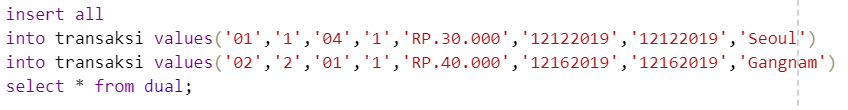
\includegraphics[width=.8\textwidth]{figure/26.PNG}
\end{center}
\item terakhir memasukkan data ke tabel transaksi dengan menggunakan fungsi insert.
\begin{center}
    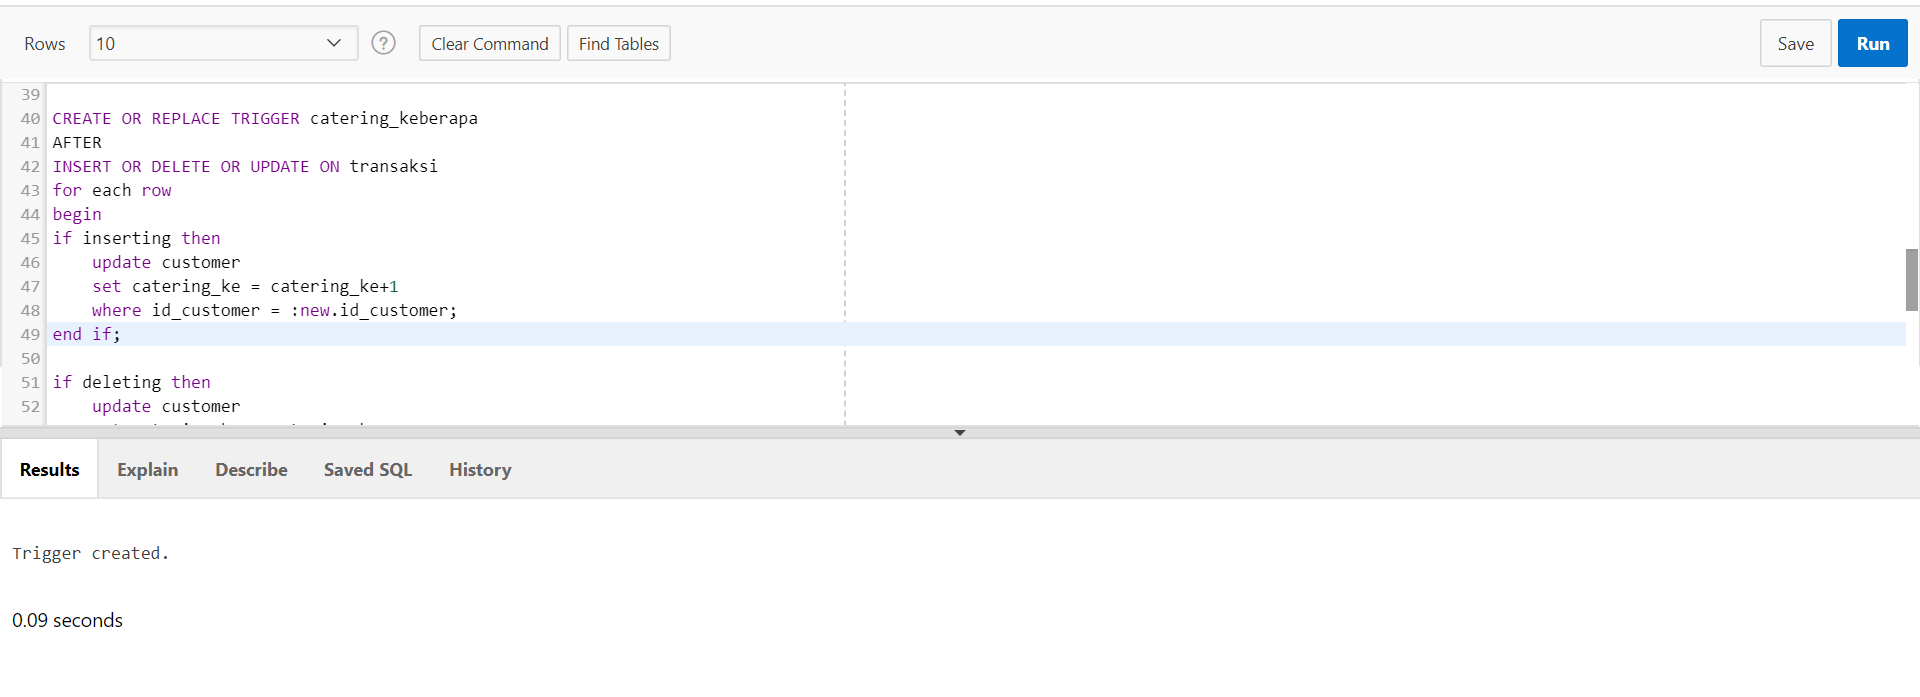
\includegraphics[width=.8\textwidth]{figure/27.PNG}
\end{center}
\item  setelah semua tabel terbuat,dan juga telah dimasukkan datanya saran saya untuk mengecek lagi cek kembali tabel anda jika primary key hingga foreigen key telah terdapat dalam table selanjutnya yang kita buat adalah membuat trigger. penjelasan mengenai trigger, jadi trigger dalam database adalah kode prosedural yang secara otomatis dijalankan untuk menanggapi perubahan tertentu pada table tertentu atau tampilan dalam database. Idealnya, Trigger harus dipertimbangkan ketika kode ini digunakan untuk mengotomatisasi perubahan yang spesifik untuk database atau pengelolaan data. Log audit adalah contoh penerapan dari Trigger. setelah mengetahui arti da fungsi trigger maka selanjutnya adalah membuat trigger pada SQL Command dengan query seperti pada gambar diatas.setelah trigger telah dibuat maka data akan secara otomatis dapat bertambah atau dapat update,delete,insert secara otomatis.
\begin{center}
    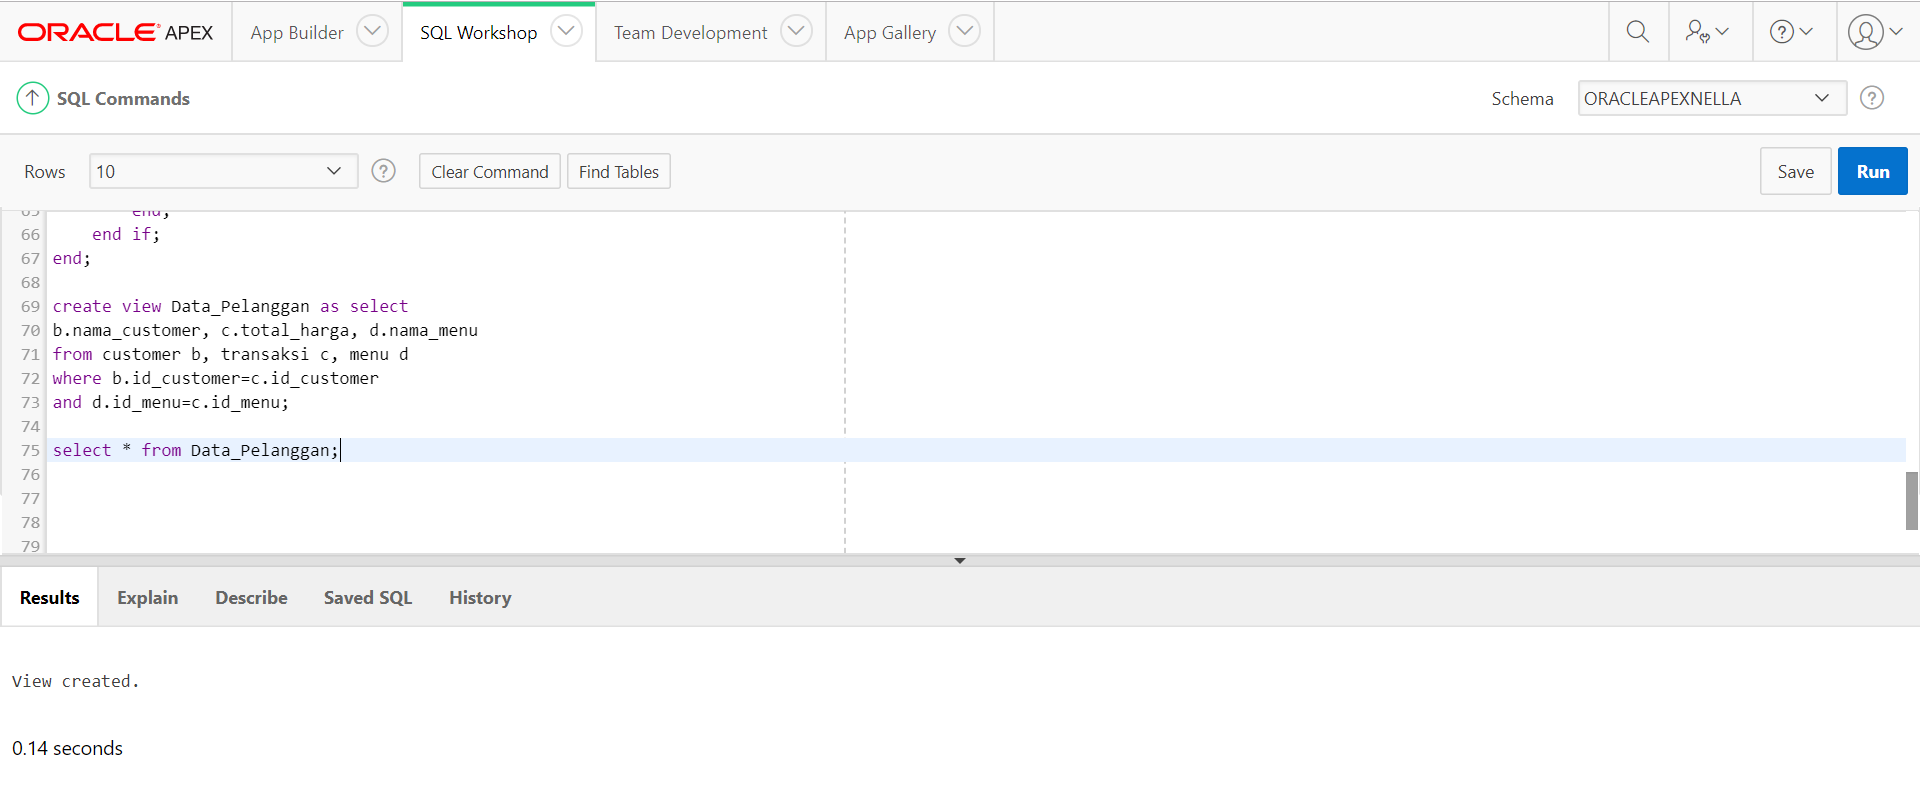
\includegraphics[width=.8\textwidth]{figure/28.PNG}
\end{center} 
\item setelah fungsi trigger telah berhasil dilakukan maka setelah itu, kita bisa menggunakan perintah atau query lain yaitu dengan CREATE VIEW, dimana perintah ini berfungsi menampilkan table yang isinya diambil dari tabel tabel yang sudah ada.
\begin{center}
    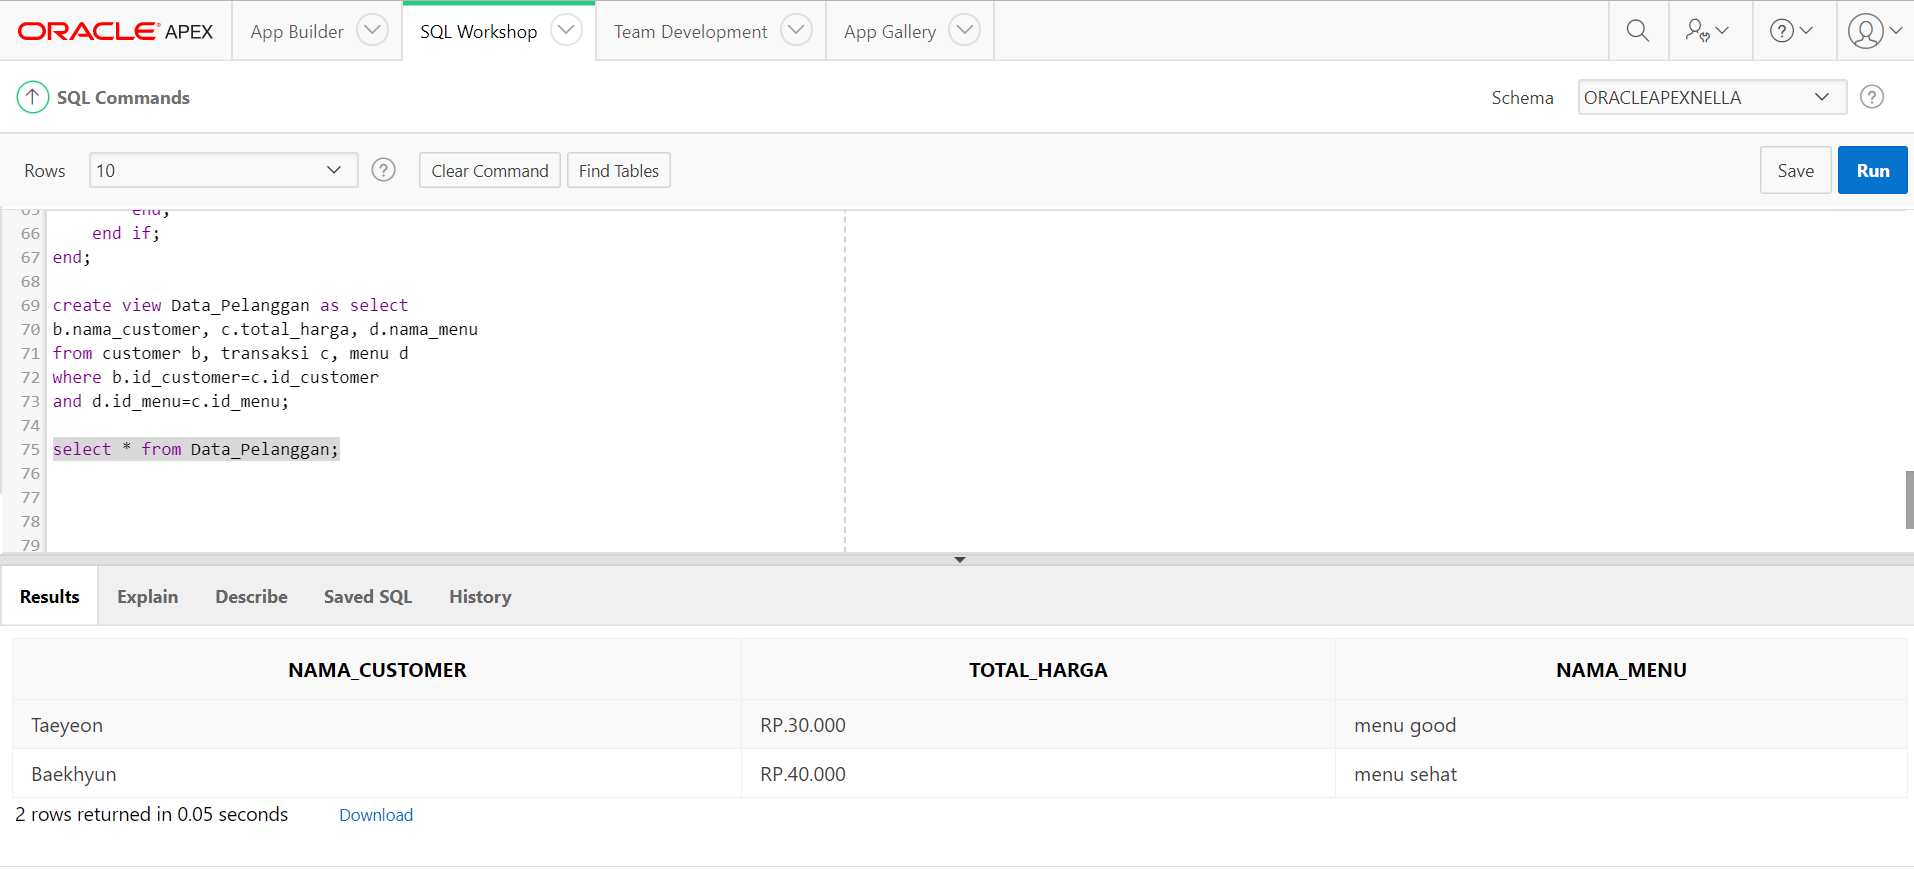
\includegraphics[width=.8\textwidth]{figure/29.PNG}
\end{center} 
\item ketika semua telah barhasil selanjutnya kita akan membuat aplikasi catering pada aplikasi apex
\end{enumerate}
\section{Pembuatan Aplikasi Catering}
\begin{enumerate}
\item langkah pertama untuk pembuatan aplikasi yaitu pada menu app builder pilih menu create.
    \begin{center}
    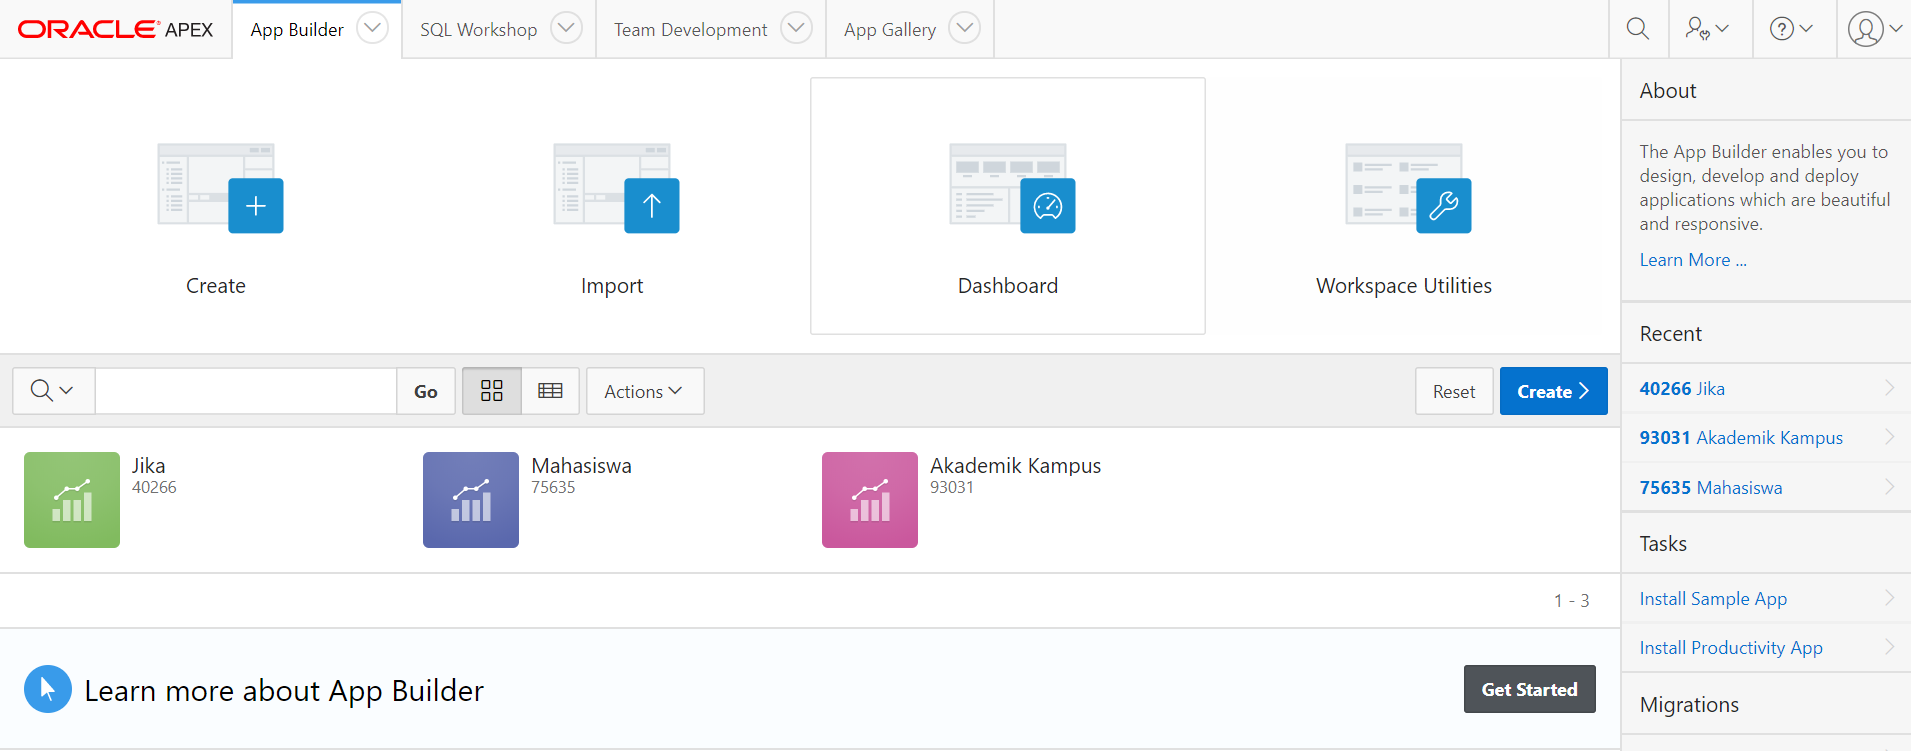
\includegraphics[width=.8\textwidth]{figure/1.PNG}
\end{center} 
\item setelah memilih menu create selanjutnya pilih menu new application untuk membuat aplikasi baru.
\begin{center}
    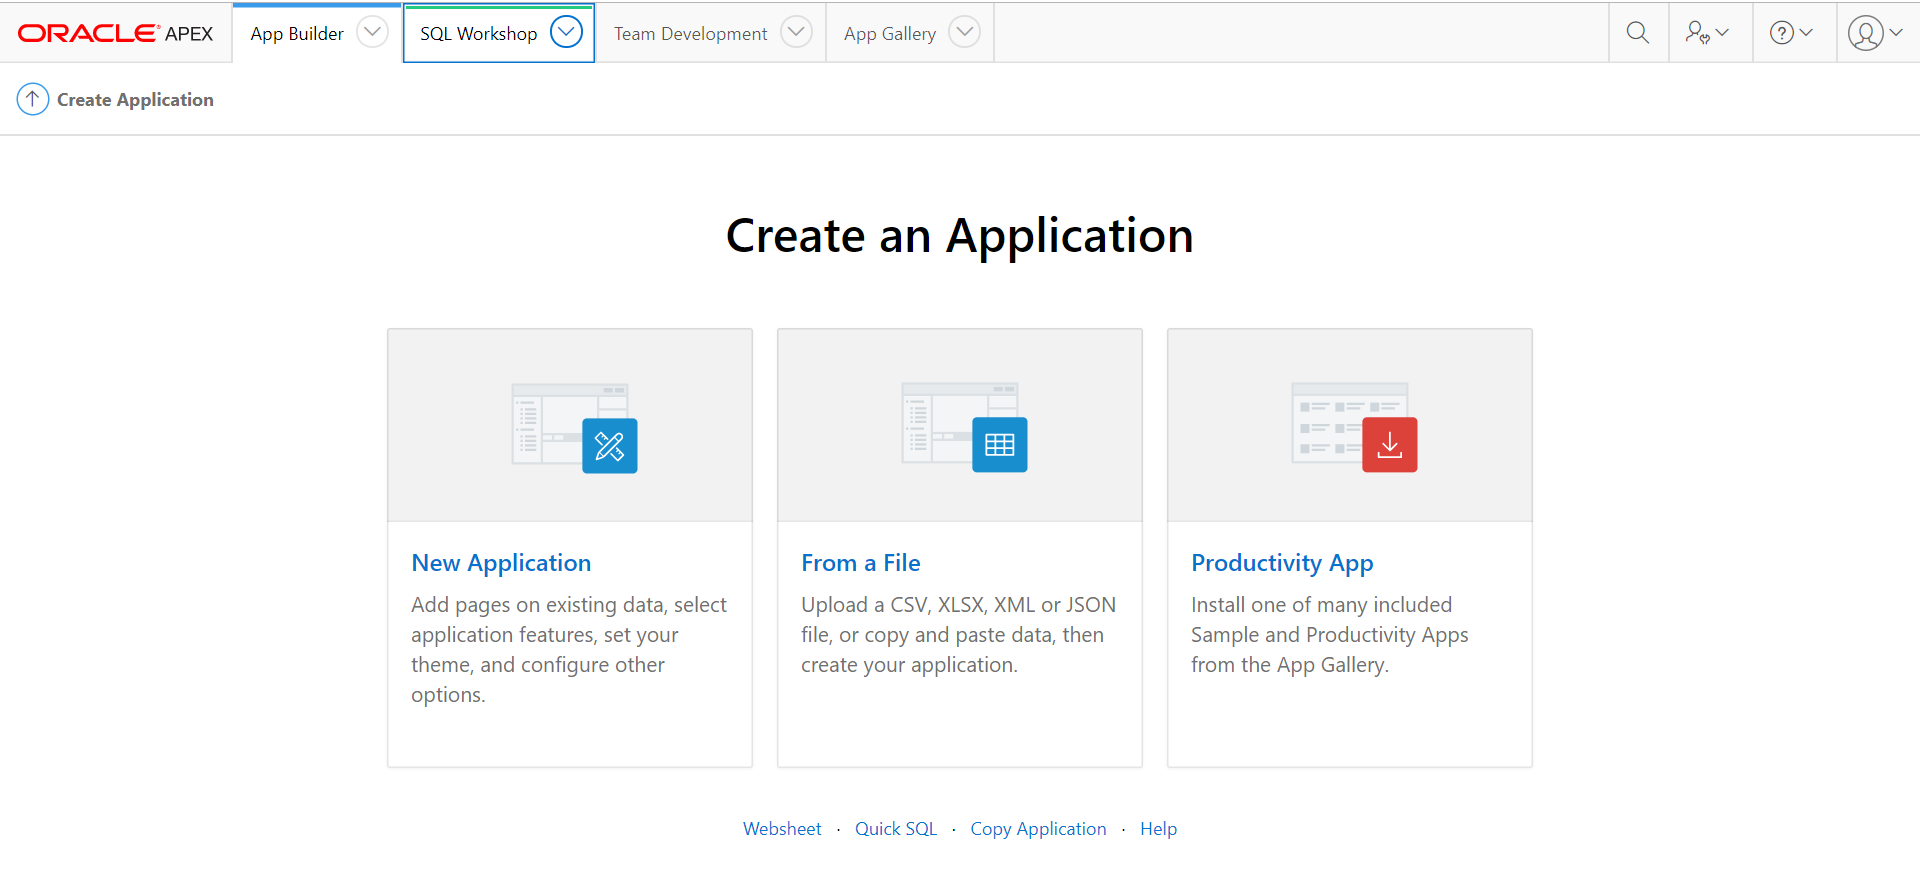
\includegraphics[width=.8\textwidth]{figure/2.PNG}
\end{center} 
\item selanjutnya membuat nama aplikasi pada form yang telah di tempat yang telah ditentukan.
\begin{center}
    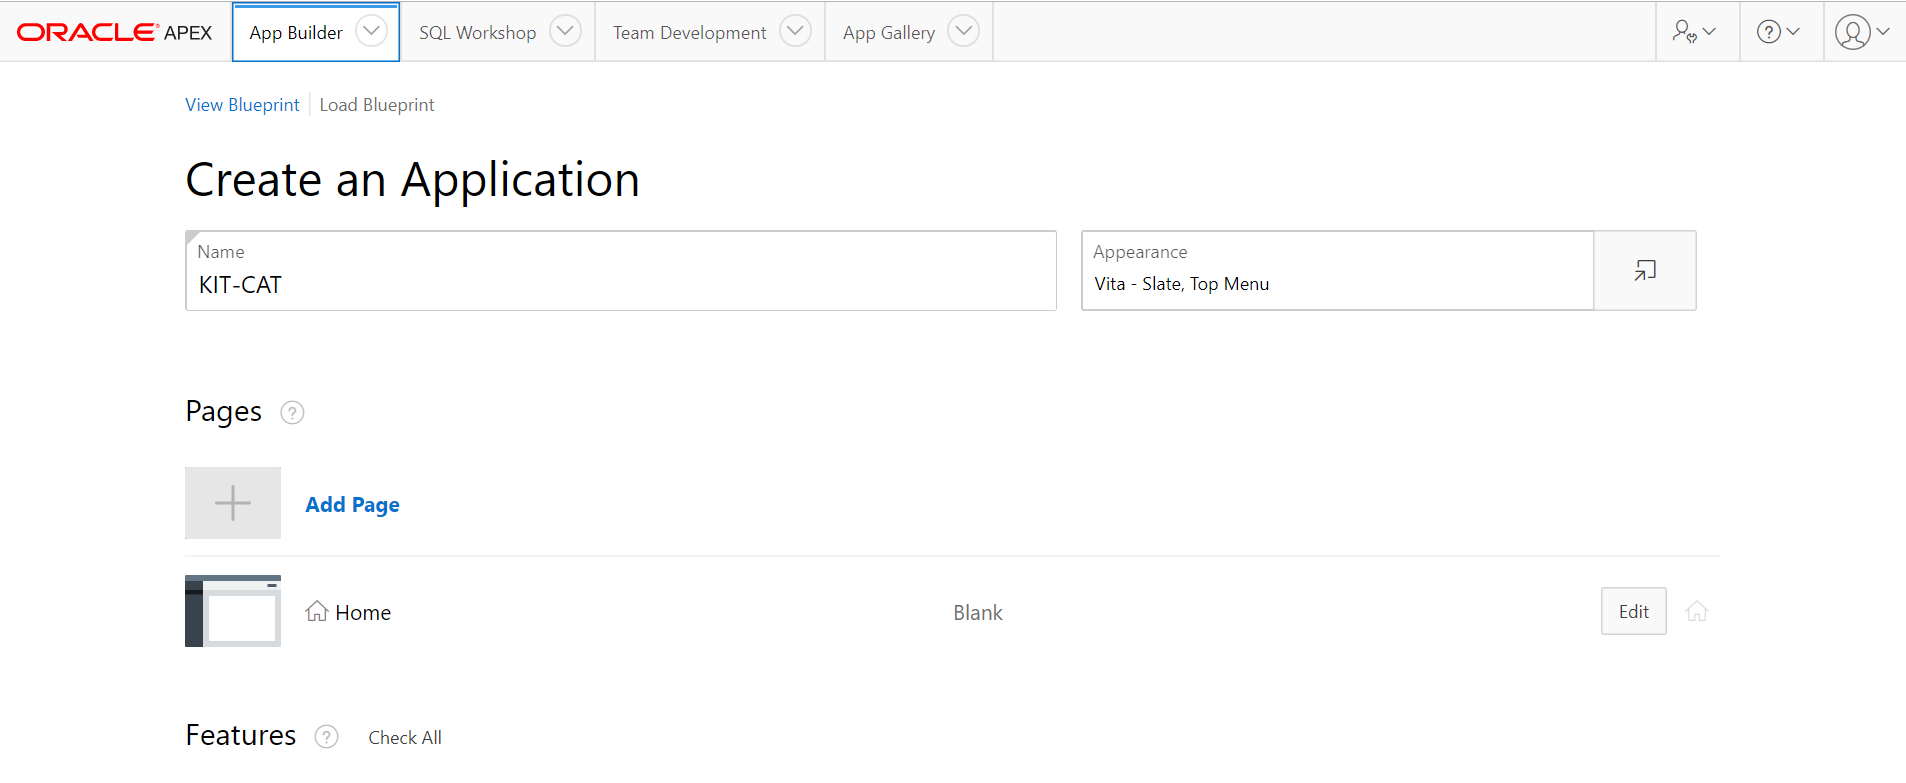
\includegraphics[width=.8\textwidth]{figure/3.PNG}
\end{center}
\item setelah nama aplikasi telah dibuat,selanjutnya yaitu membuat menu pada aplikasi seperti gambar dibawa ini.disini saya memilih menu interactive menu.
\begin{center}
    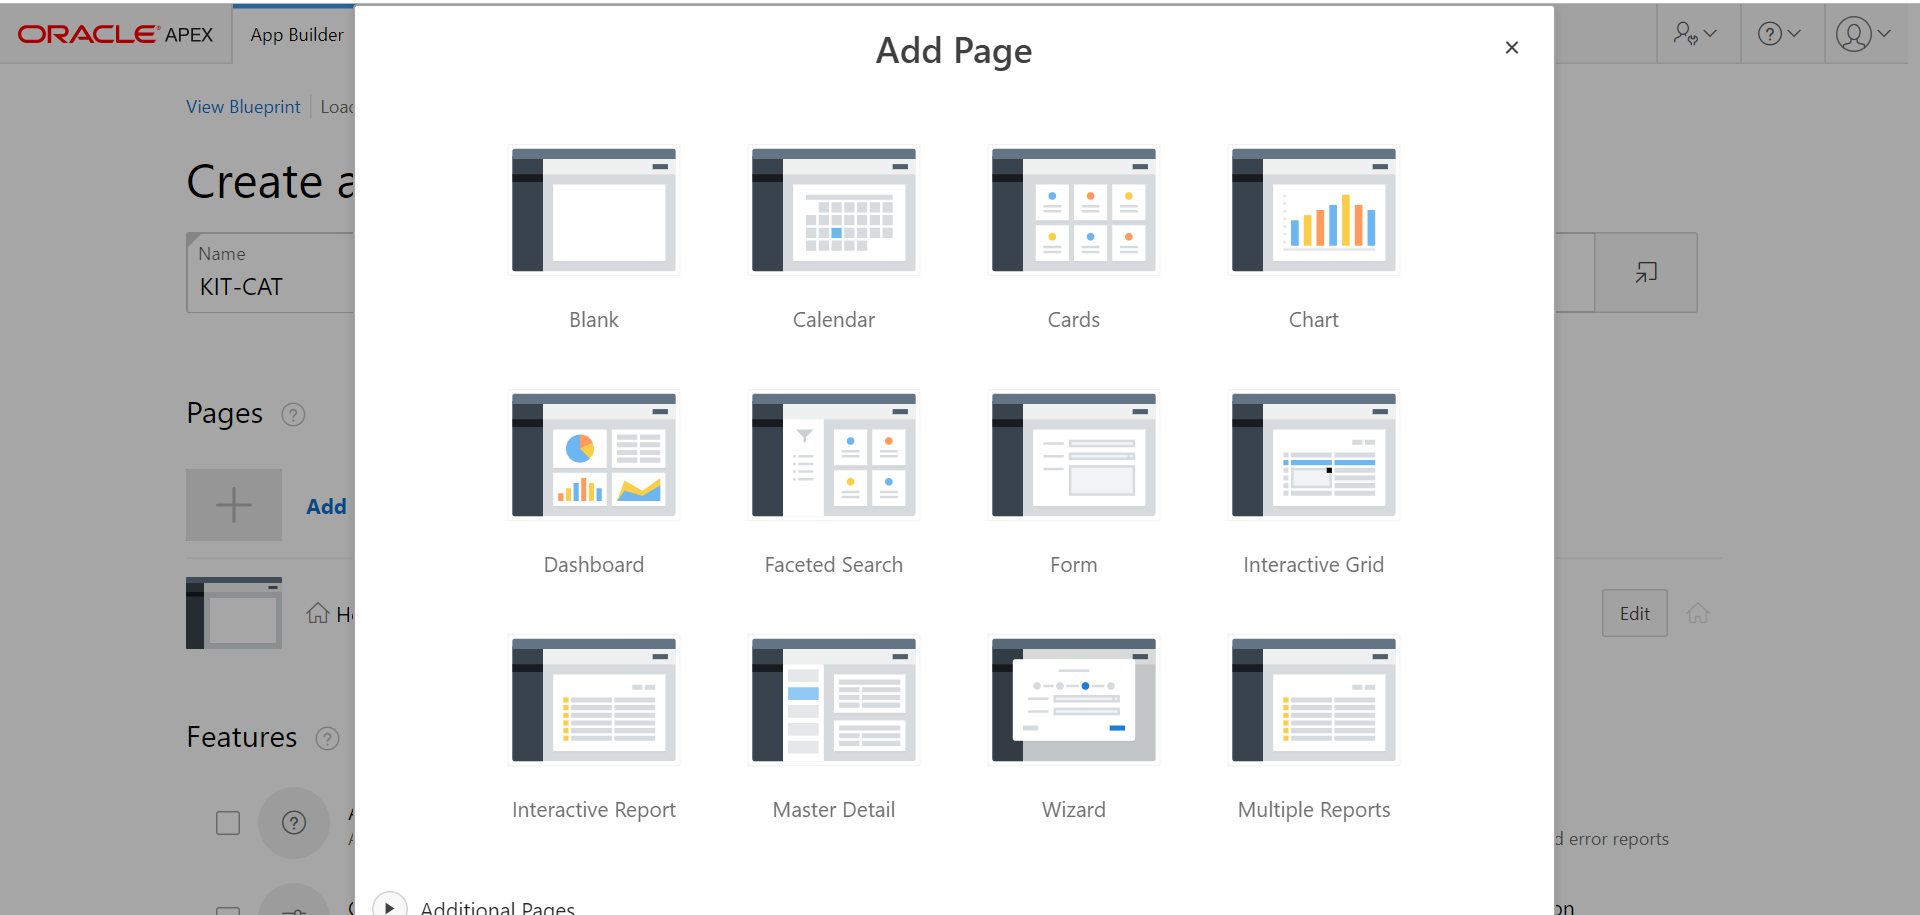
\includegraphics[width=.8\textwidth]{figure/4.PNG}
\end{center}
\item setelah itu pilih tabel yang akan akan dimasukkan pada menu.lalu add page.ulang langkah ini sampai menu telah selesai semua.
\begin{center}
    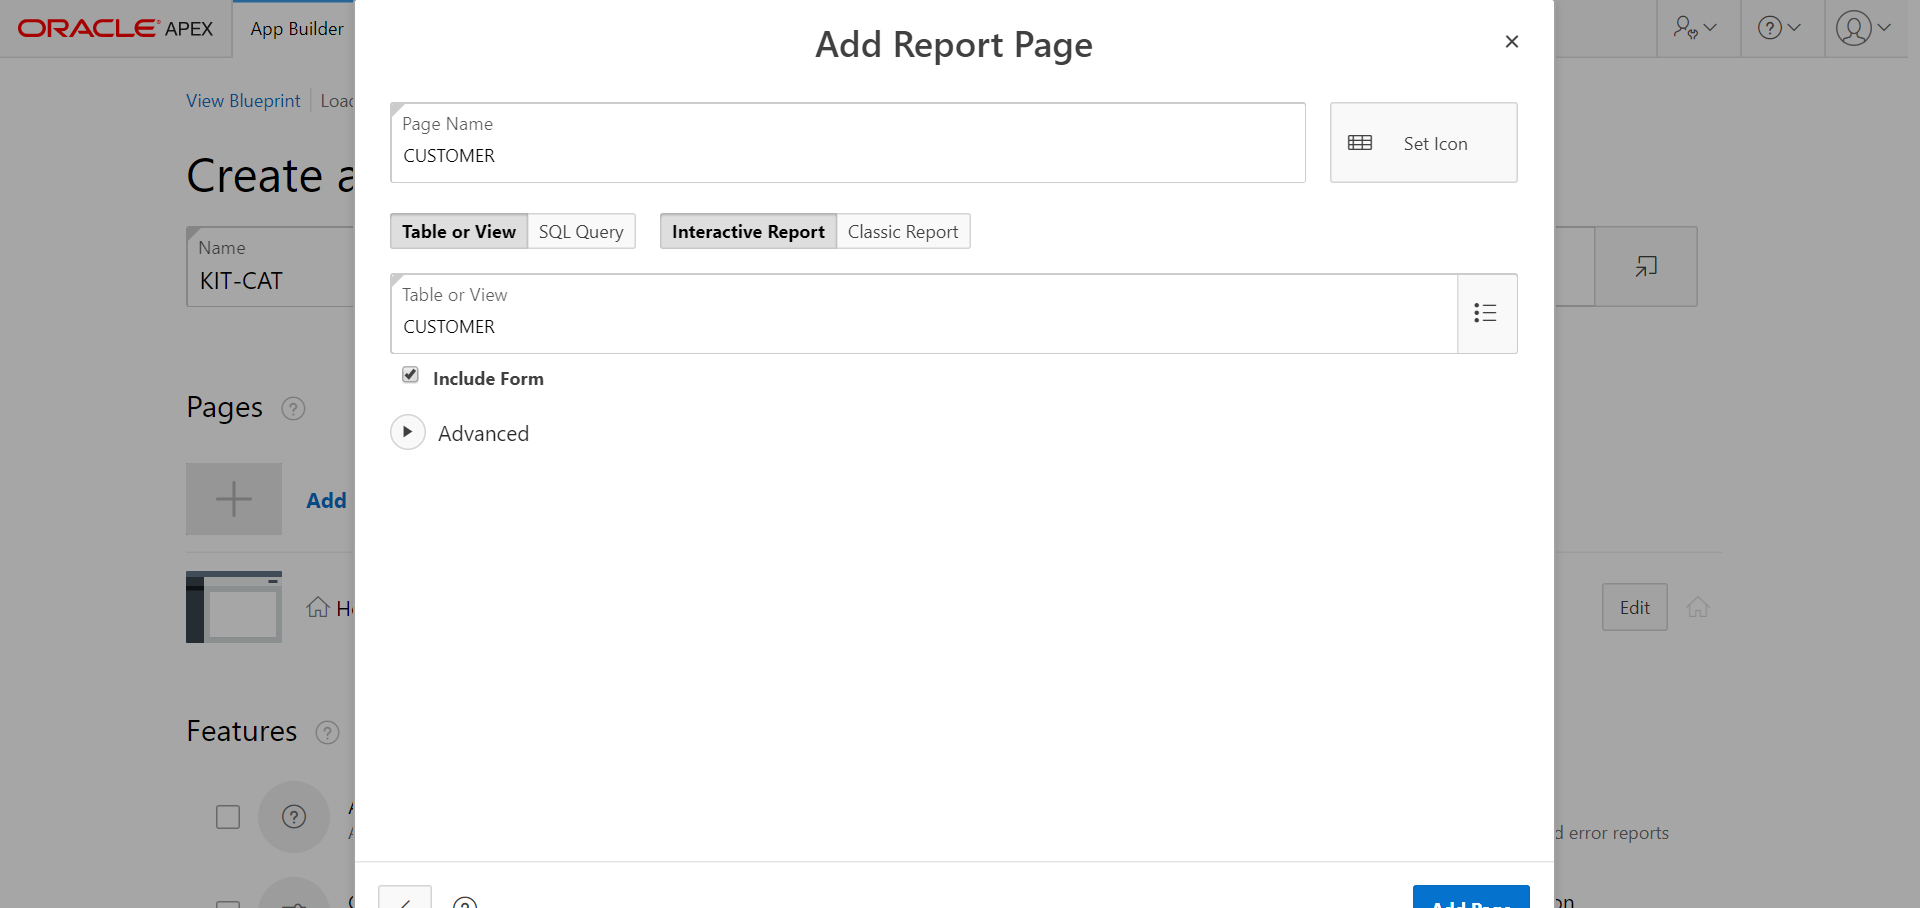
\includegraphics[width=.8\textwidth]{figure/5.PNG}
\end{center}
\item setelah selesai membuat menu selanjutnya adalah membuat aplikasi yaitu klik create application sehinnga aplikasi kita akan dibuat.
\begin{center}
    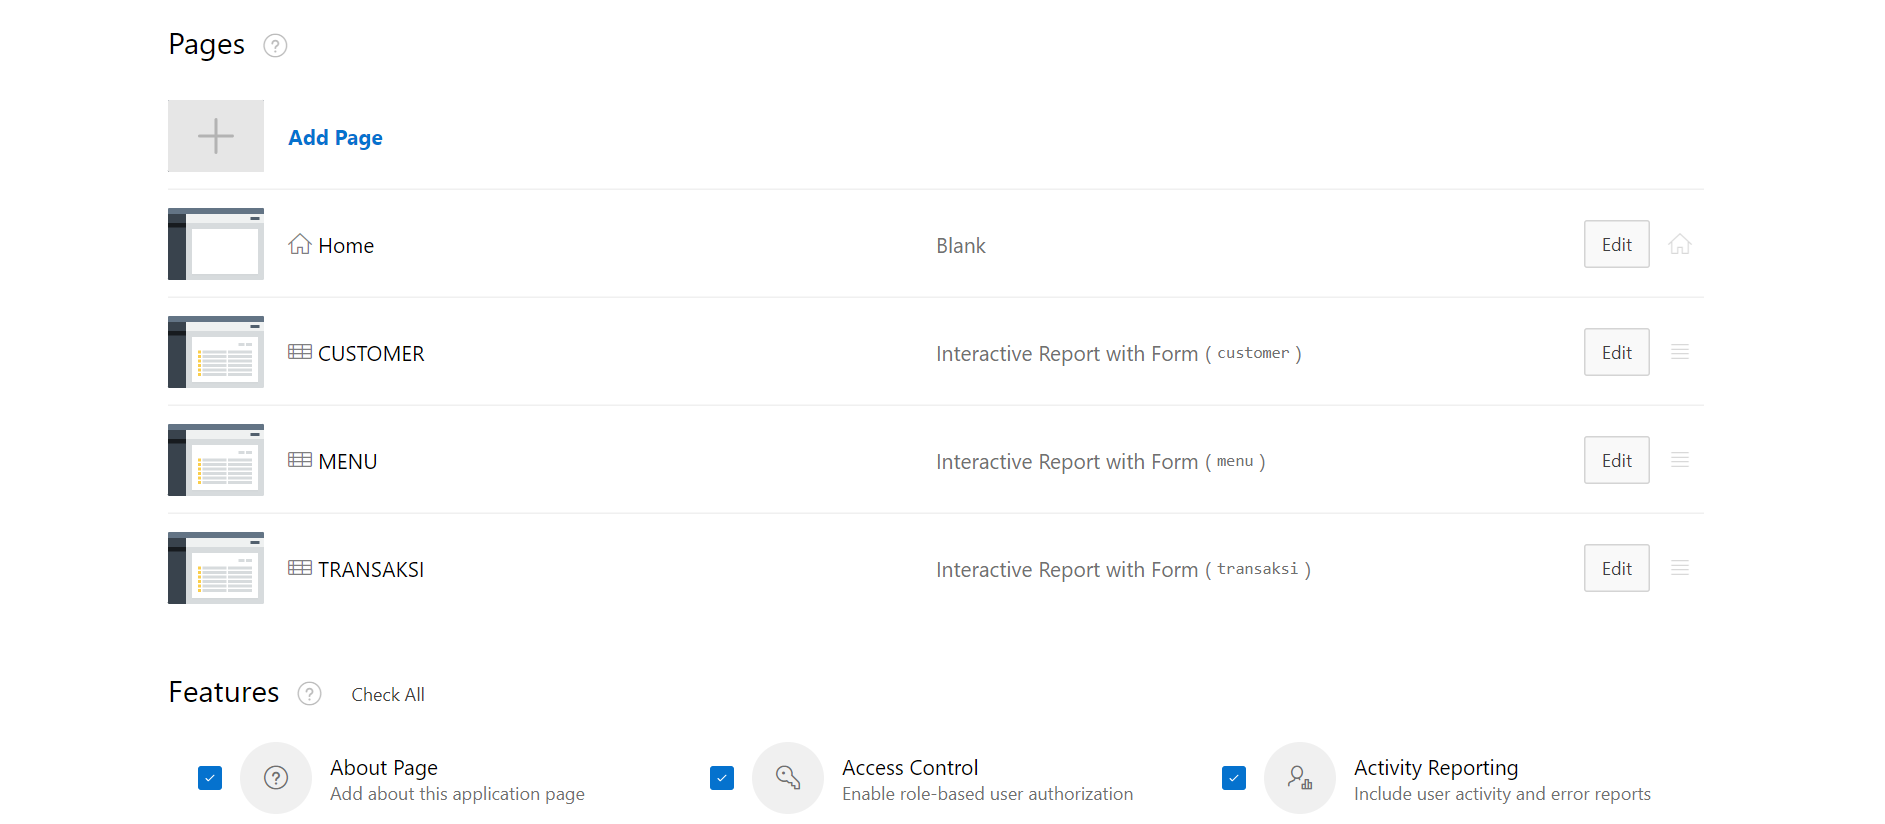
\includegraphics[width=.8\textwidth]{figure/6.PNG}
\end{center}
\begin{center}
    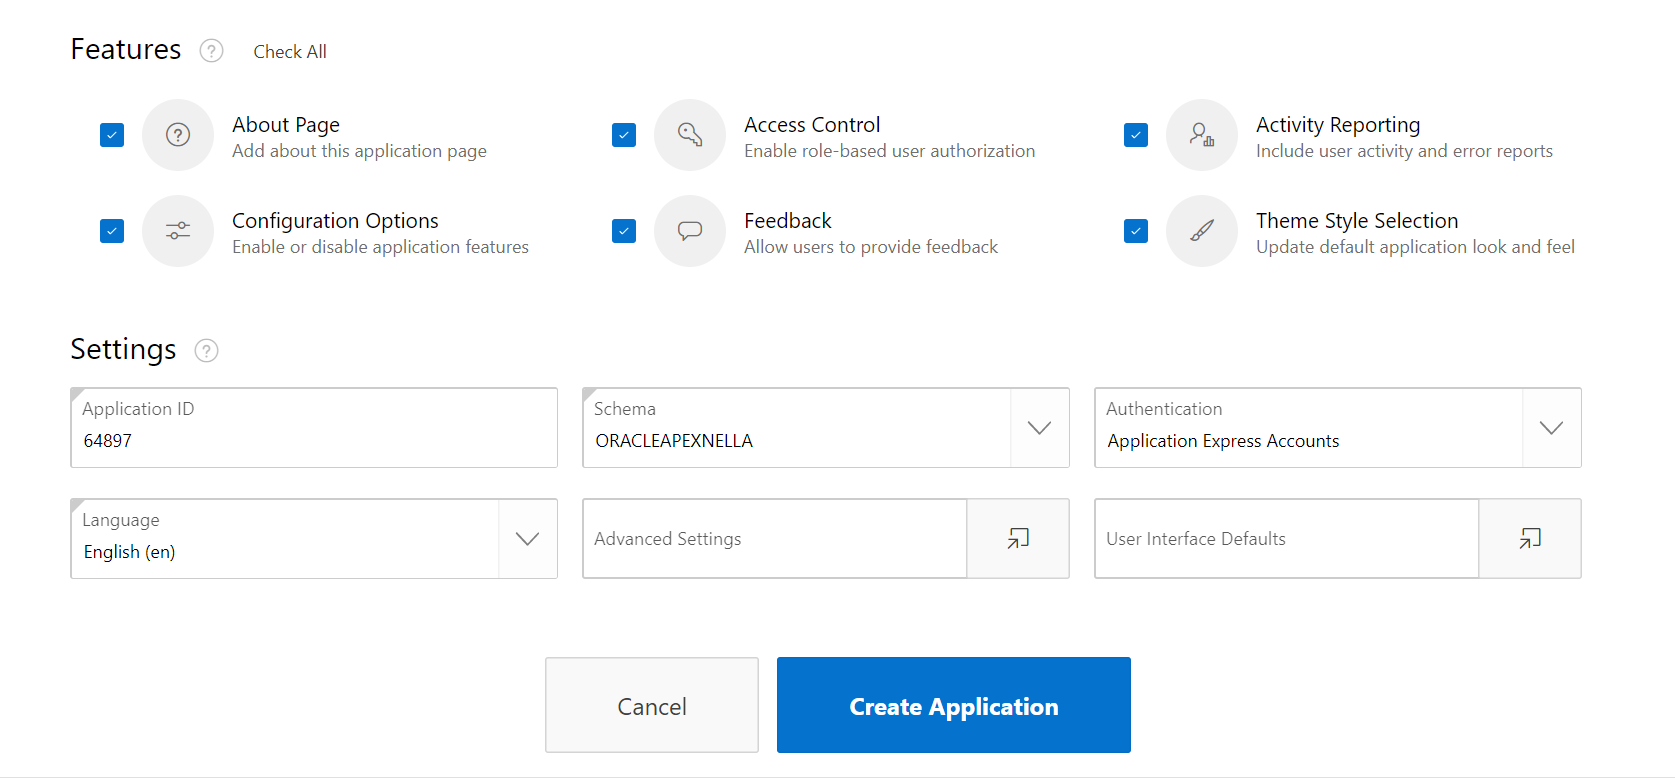
\includegraphics[width=.8\textwidth]{figure/7.PNG}
\end{center}
\begin{center}
    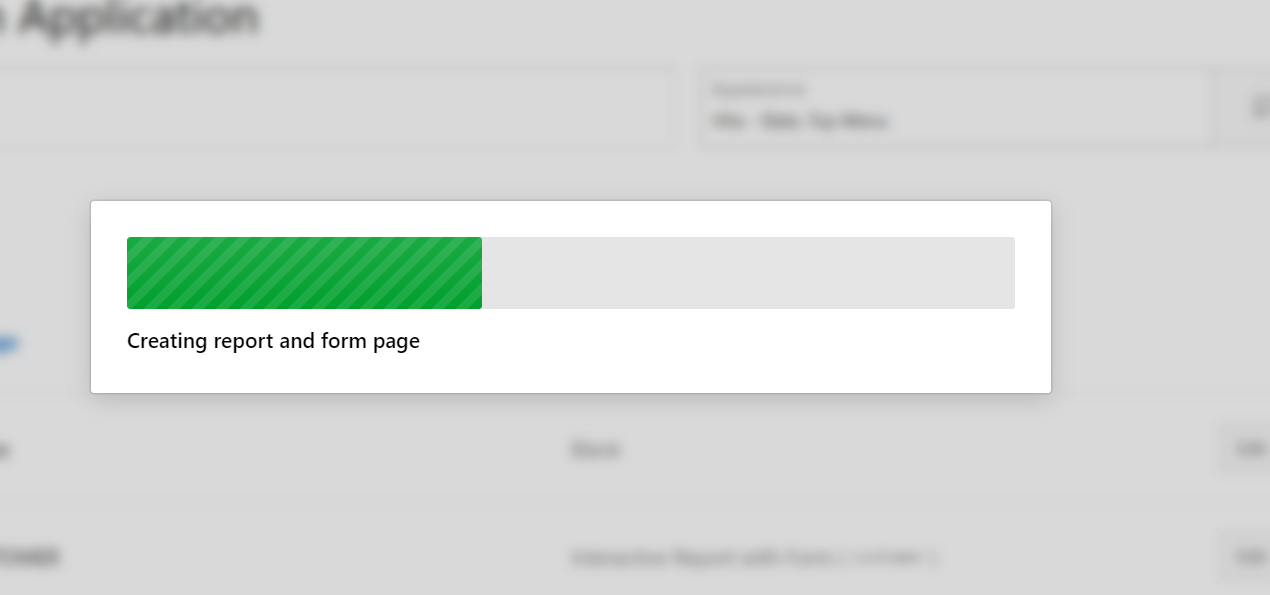
\includegraphics[width=.8\textwidth]{figure/8.PNG}
\end{center}
\item jika telah berhasil maka aplikasi telah dibuat.selanjutnya adalah menjalankan aplikasi.
\begin{center}
    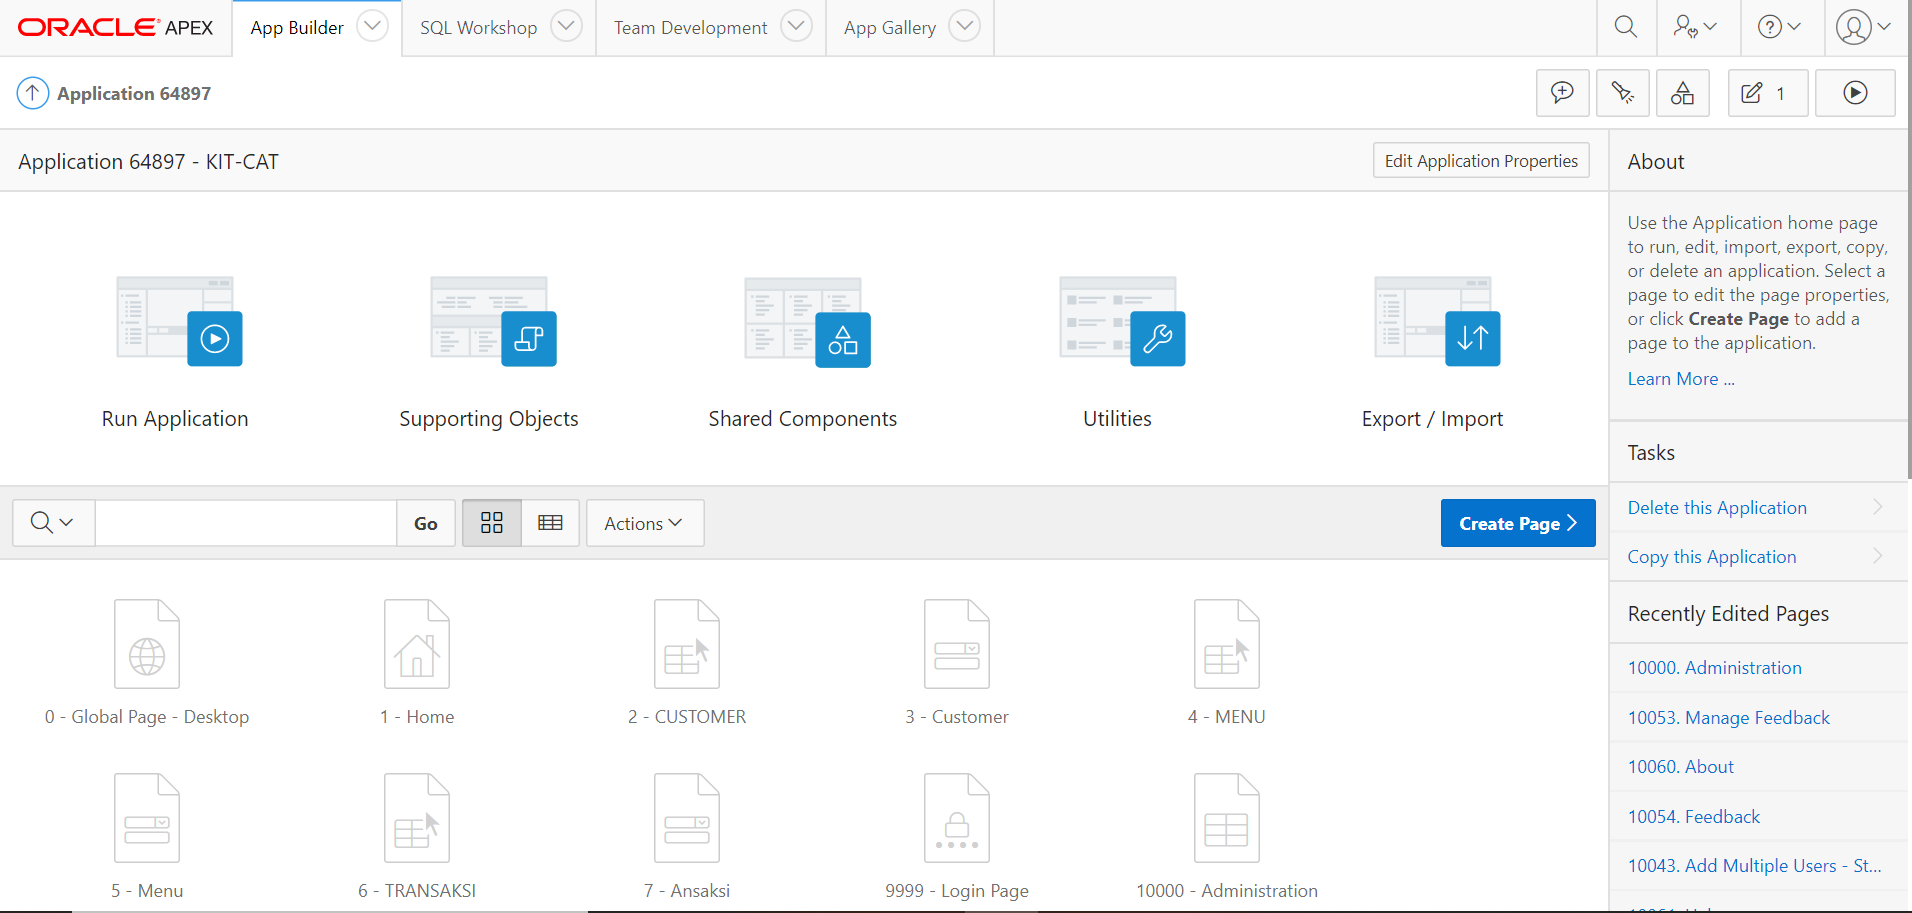
\includegraphics[width=.8\textwidth]{figure/9.PNG}
\end{center}
\item masukkan data anda
\begin{center}
    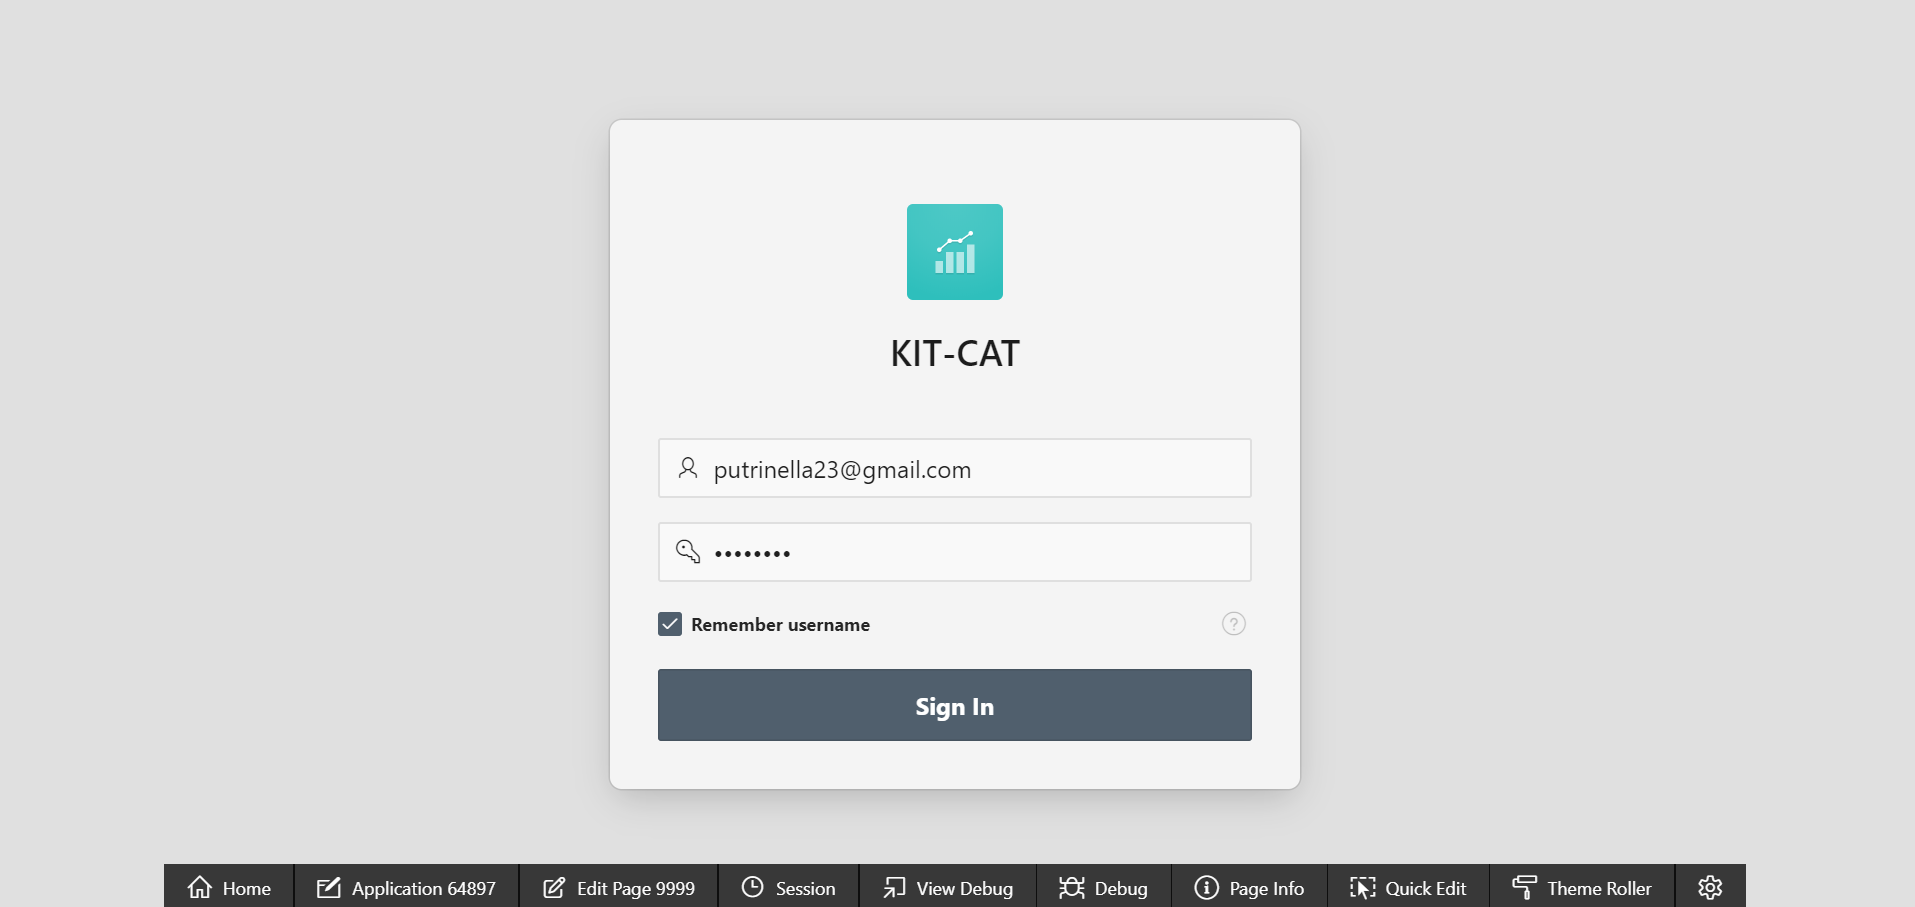
\includegraphics[width=.8\textwidth]{figure/10.PNG}
\end{center}
\item tampilan menu utama aplikasi kita.
\begin{center}
    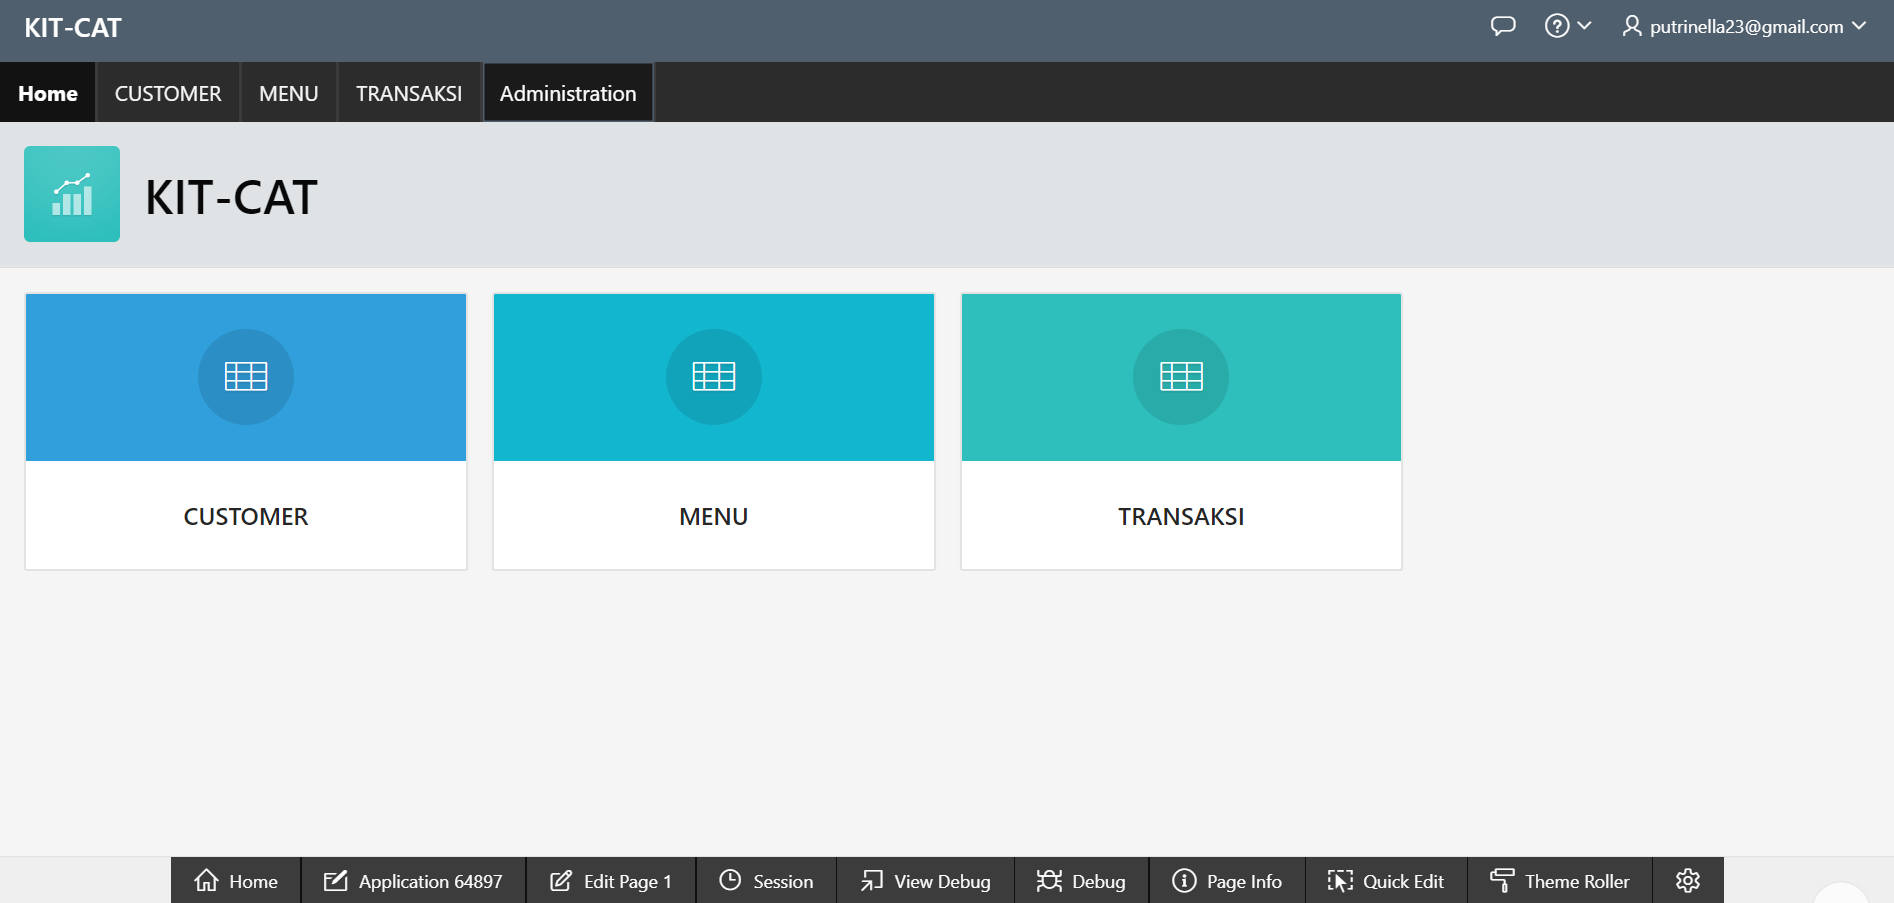
\includegraphics[width=.8\textwidth]{figure/11.PNG}
\end{center}
untuk menguji trigger maka kita dapat mengujinya
\begin{center}
    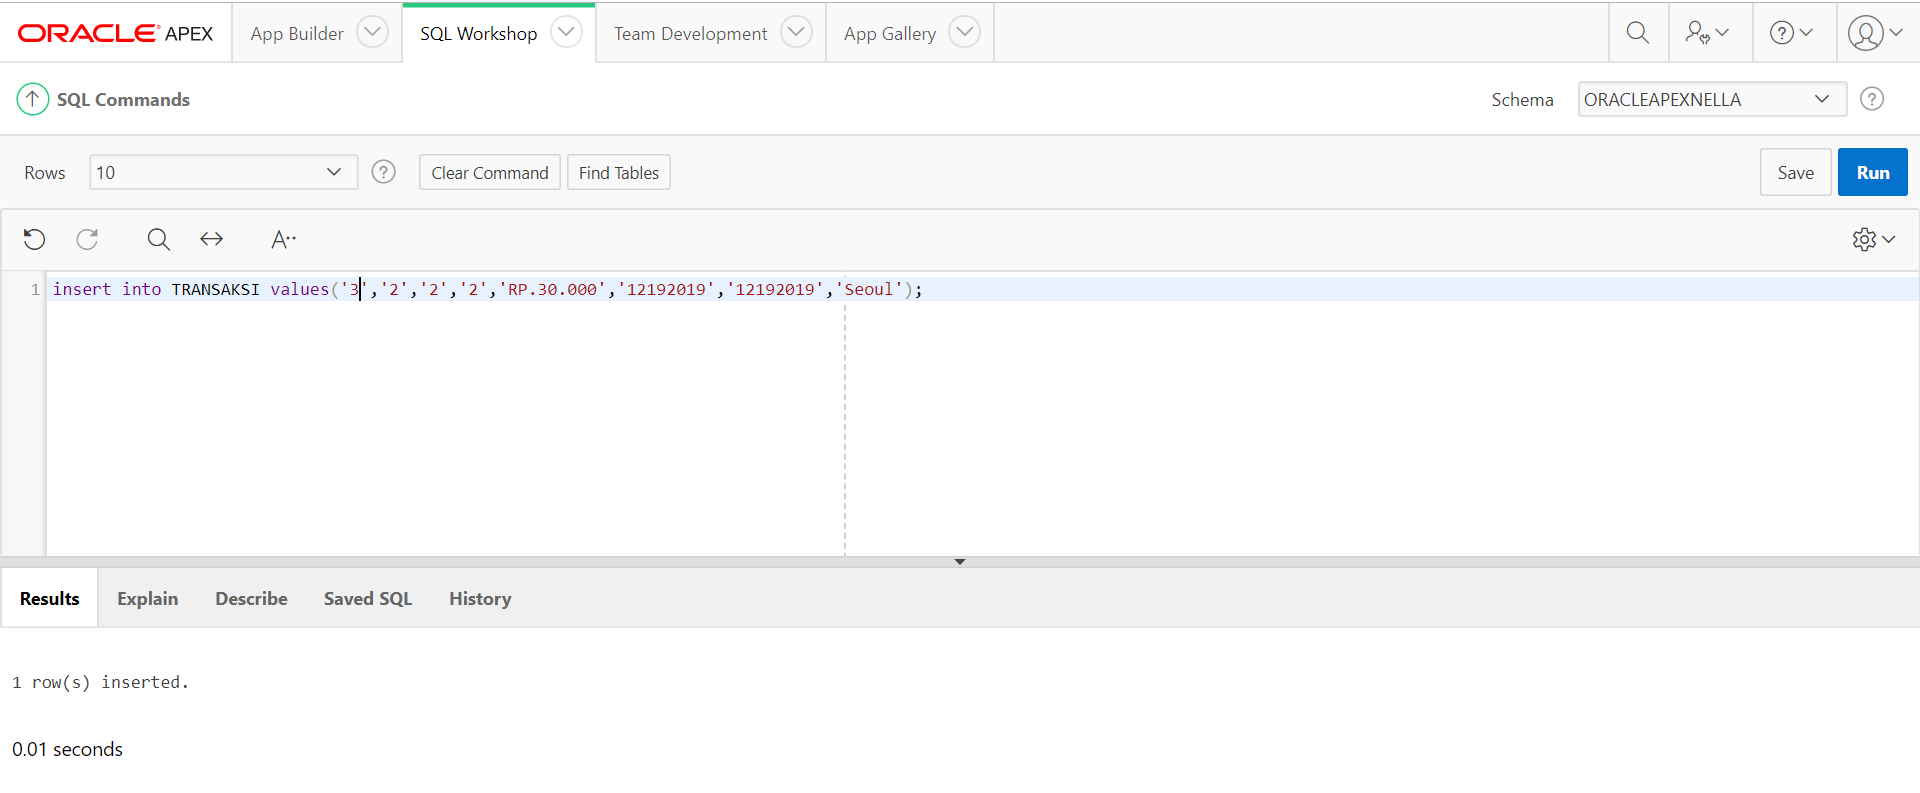
\includegraphics[width=.8\textwidth]{figure/12.PNG}
\end{center}
\item maka secara otomatis data akan mengupdate sendiri 
\begin{center}
    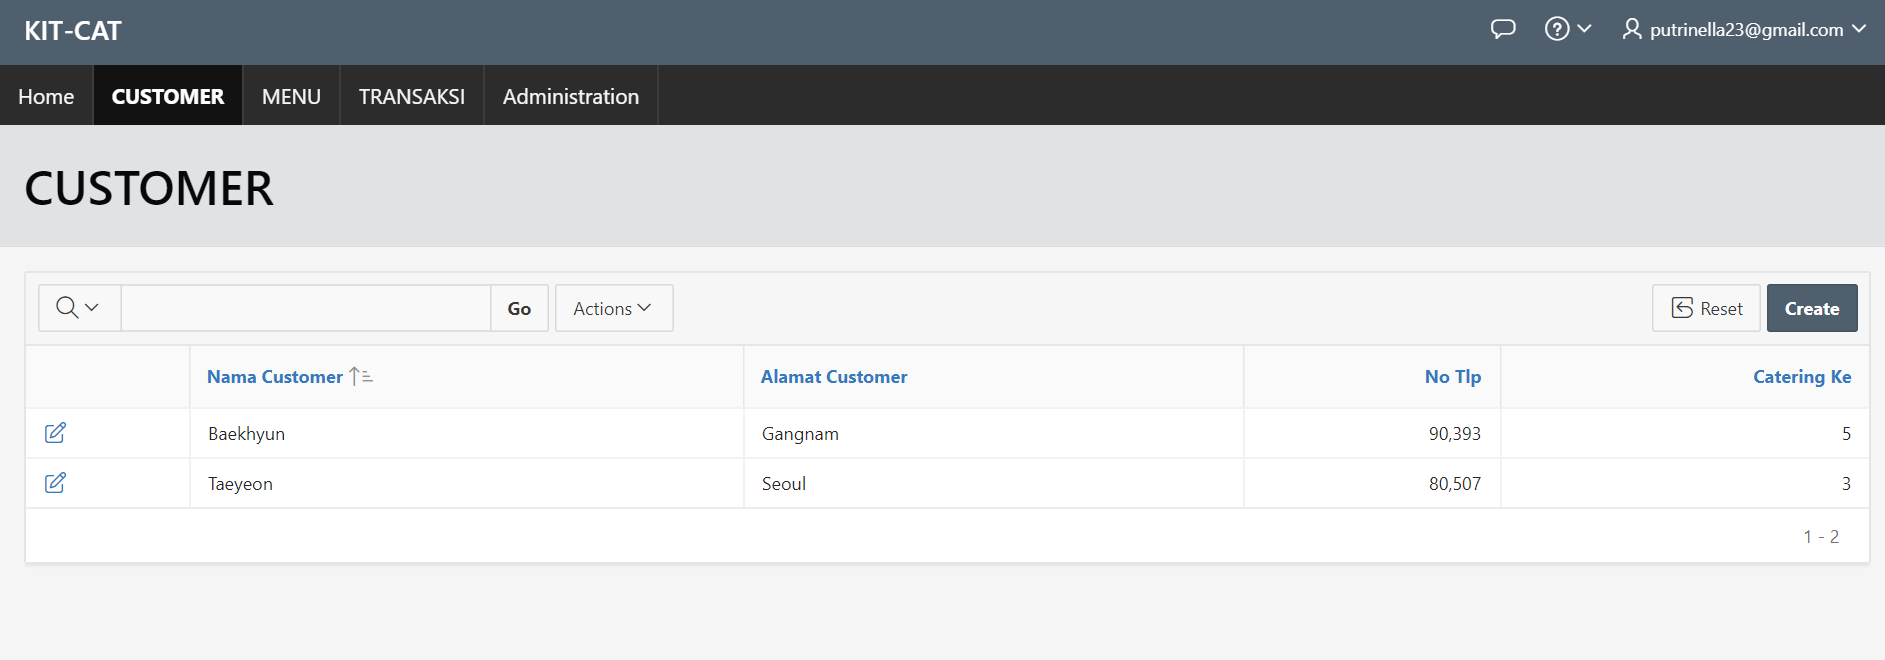
\includegraphics[width=.8\textwidth]{figure/13.PNG}
\end{center}
\begin{center}
    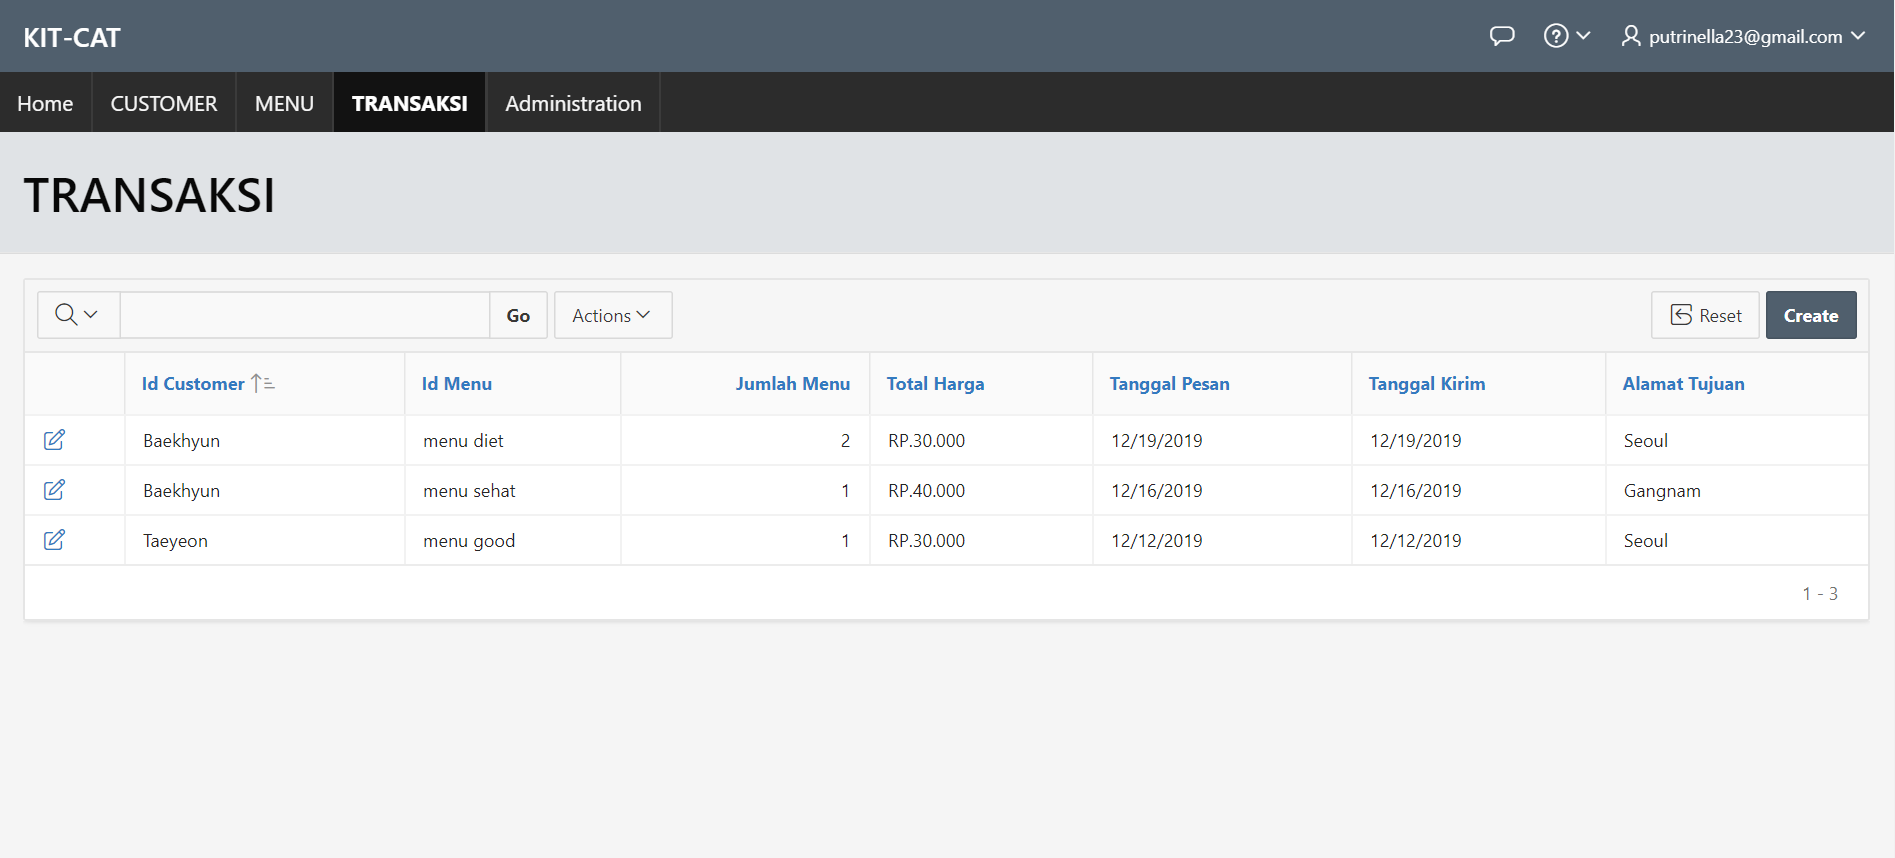
\includegraphics[width=.8\textwidth]{figure/14.PNG}
\end{center}
SELESAI\\
LINK : https://apex.oracle.com/pls/apex/f?p=64897:LOGIN_DESKTOP:714946124241378::::: \\
USERNAME : putrinella23@gmail.com \\
PASSWORD : nella118
\end{enumerate}
\end{document}

